\documentclass[10pt,portrait,final,a1paper,fontscale=0.51]{baposter}
\usepackage[utf8]{inputenc}
\usepackage[spanish]{babel}
\usepackage{calc}
%----------------------------------------Paquetes para graficos---------------------------------------%
    \usepackage{graphicx}	% para incluir graficos

    
    \usepackage[pdf]{pstricks}
    \usepackage{auto-pst-pdf}
%     \usepackage{pst-node}
%     \usepackage{pst-plot}
%     \usepackage{multido}
%     \usepackage{pst-func}
%     \usepackage{pst-eucl}
%     \usepackage{pst-3dplot} % pst 3D
%     \usepackage{auto-pst-pdf}
%     \usepackage{epstopdf}
    
\usepackage{amsmath}
\usepackage{amssymb}
\usepackage{relsize}
\usepackage{multirow}
\usepackage{rotating}
\usepackage{bm}
\usepackage{enumitem}
\usepackage{url}
\usepackage{booktabs}

\usepackage{graphicx}
\usepackage{multicol}

%\usepackage{times}
%\usepackage{helvet}
%\usepackage{bookman}
% \setlength{\parindent}{0pt}
\usepackage{palatino}
\setlength\parindent{0pt}	
\newcommand{\captionfont}{\footnotesize}

\graphicspath{{images/}{../images/}}
\usetikzlibrary{calc}


\newcommand{\Matrix}[1]{\begin{bmatrix} #1 \end{bmatrix}}
\newcommand{\Vector}[1]{\begin{pmatrix} #1 \end{pmatrix}}

\newcommand*{\norm}[1]{\mathopen\| #1 \mathclose\|}% use instead of $\|x\|$
\newcommand*{\abs}[1]{\mathopen| #1 \mathclose|}% use instead of $\|x\|$
\newcommand*{\normLR}[1]{\left\| #1 \right\|}% use instead of $\|x\|$

\newcommand*{\SET}[1]  {\ensuremath{\mathcal{#1}}}
\newcommand*{\FUN}[1]  {\ensuremath{\mathcal{#1}}}
\newcommand*{\MAT}[1]  {\ensuremath{\boldsymbol{#1}}}
\newcommand*{\VEC}[1]  {\ensuremath{\boldsymbol{#1}}}
\newcommand*{\CONST}[1]{\ensuremath{\mathit{#1}}}

\DeclareMathOperator*{\argmax}{arg\,max}
\DeclareMathOperator*{\diag}{diag}
\DeclareMathOperator*{\argmin}{arg\,min}
\DeclareMathOperator*{\vectorize}{vec}
\DeclareMathOperator*{\reshape}{reshape}

%\font\dsfnt=dsrom12

\newcommand{\SNN}{\ensuremath{\mathbb N}}
\newcommand{\SRR}{\ensuremath{\mathbb R}}
\newcommand{\SZZ}{\ensuremath{\mathbb Z}}
%-----------------------------------------------------------------------------
% Matrices of the shape model
\renewcommand{\a}{\VEC\alpha}
\renewcommand{\v}{\VEC v}
\renewcommand{\l}{\VEC l}
\newcommand*{\m}{\VEC{\mu}}
\newcommand*{\M}{\MAT{M}}
\renewcommand*{\P}{\MAT{\Pi}}

%\newcommand{\J}{\SET J}
\newcommand{\J}{\SET{P}}
\newcommand{\Active}{\mathcal{A}}
\newcommand{\Selection}{\mathbf{S}}
\newcommand{\AllSelections}{\mathfrak{S}}
\newcommand{\Params}{\VEC\Theta}

%%%%%%%%%%%%%%%%%%%%%%%%%%%%%%%%%%%%%%%%%%%%%%%%%%%%%%%%%%%%%%%%%%%%%%%%%%%%%%%%
%%%% Some math symbols used in the text
%%%%%%%%%%%%%%%%%%%%%%%%%%%%%%%%%%%%%%%%%%%%%%%%%%%%%%%%%%%%%%%%%%%%%%%%%%%%%%%%

%%%%%%%%%%%%%%%%%%%%%%%%%%%%%%%%%%%%%%%%%%%%%%%%%%%%%%%%%%%%%%%%%%%%%%%%%%%%%%%%
% Multicol Settings
%%%%%%%%%%%%%%%%%%%%%%%%%%%%%%%%%%%%%%%%%%%%%%%%%%%%%%%%%%%%%%%%%%%%%%%%%%%%%%%%
\setlength{\columnsep}{1.5em}
\setlength{\columnseprule}{0mm}

%%%%%%%%%%%%%%%%%%%%%%%%%%%%%%%%%%%%%%%%%%%%%%%%%%%%%%%%%%%%%%%%%%%%%%%%%%%%%%%%
% Save space in lists. Use this after the opening of the list
%%%%%%%%%%%%%%%%%%%%%%%%%%%%%%%%%%%%%%%%%%%%%%%%%%%%%%%%%%%%%%%%%%%%%%%%%%%%%%%%
\newcommand{\compresslist}{%
\setlength{\itemsep}{1pt}%
\setlength{\parskip}{0pt}%
\setlength{\parsep}{0pt}%
}
\def\minus{%
  \setbox0=\hbox{-}%
  \vcenter{%
    \hrule width\wd0 height \the\fontdimen8\textfont3%
  }%
}
\newcommand{\no}{\noindent}
\newcommand{\dis}{\displaystyle}
%
\newcommand{\CC}{\mathbb{C}}
\newcommand{\RR}{\mathbb{R}}
\newcommand{\NN}{\mathbb{N}}
\newcommand{\ZZ}{\mathbb{Z}}
\newcommand{\Z}{\mathbb{Z}}
\newcommand{\PP}{\mathcal{P}}
\newcommand{\MM}{\mathcal{M}}
%
\newcommand{\CN}{\mathbb{C}^n}
\newcommand{\CM}{\mathbb{C}^m}
\newcommand{\RN}{\mathbb{R}^n}
\newcommand{\RM}{\mathbb{R}^m}
%
\newcommand{\CNN}{\CC^{n \times n}}
\newcommand{\CMM}{\CC^{m \times m}}
\newcommand{\CMN}{\CC^{m \times n}}
\newcommand{\RNN}{\RR^{n \times n}}
\newcommand{\RMM}{\RR^{m \times m}}
%
\newcommand{\Or}{\mathcal{O}}
%
\newcommand{\medio}{\frac{1}{2}}
\newcommand{\cuarto}{\frac{1}{4}}
\newcommand{\octavo}{\frac{1}{8}}
\newcommand{\trescuartos}{\frac{3}{4}}
%
\newcommand{\dd}{\frac{dy}{dx}}
%
\newcommand{\kj}{\kappa(j)}
\newcommand{\nh}{\tilde{h}}
%
\newcommand{\implica}{\Longrightarrow}
%
\newcommand{\pic}{>_{\RRN}}
\newcommand{\picf}{>_{\RRf}}
%
\newcommand{\vx}{\vec x}
\newcommand{\vy}{\vec y}
\newcommand{\vp}{\vec p}
%
\newcommand{\vpz}{\vec{p_0}}
\newcommand{\vpo}{\vec{p_1}}
\newcommand{\vpj}{\vec{p_j}}
\newcommand{\vpk}{\vec{p_k}}
\newcommand{\vq}{\vec q}
%
\newcommand{\alz}{\alpha_0}
\newcommand{\alo}{\alpha_1}
\newcommand{\ali}{\alpha_i}
\newcommand{\alj}{\alpha_j}
\newcommand{\alk}{\alpha_k}
\newcommand{\alzas}{\alpha_0 ^*}
\newcommand{\aloas}{\alpha_1 ^*}
\newcommand{\alias}{\alpha_i ^*}
\newcommand{\aljas}{\alpha_j ^*}
\newcommand{\alkas}{\alpha_k ^*}
\newcommand{\conf}{\text{Conf}}
\newcommand{\confin}{\text{Conf}_\text{fin}}
\newcommand{\pr}{\text{pr}}
\newcommand{\msubseteq}{\trianglelefteq\hspace{-2.5pt}\sqsubseteq }
\newcommand{\alp}[1]{\Sigma^{#1}}
\renewcommand{\phi}{\varphi}
%%%%%%%%%%%%%%%%%%%%%%%%%%%%%%%%%%%%%%%%%%%%%%%%%%%%%%%%%%%%%%%%%%%%%%%%%%%%%%
%%% Begin of Document
%%%%%%%%%%%%%%%%%%%%%%%%%%%%%%%%%%%%%%%%%%%%%%%%%%%%%%%%%%%%%%%%%%%%%%%%%%%%%%

\begin{document}

%%%%%%%%%%%%%%%%%%%%%%%%%%%%%%%%%%%%%%%%%%%%%%%%%%%%%%%%%%%%%%%%%%%%%%%%%%%%%%
%%% Here starts the poster
%%%---------------------------------------------------------------------------
%%% Format it to your taste with the options
%%%%%%%%%%%%%%%%%%%%%%%%%%%%%%%%%%%%%%%%%%%%%%%%%%%%%%%%%%%%%%%%%%%%%%%%%%%%%%
% Define some colors

\definecolor{lightorange}{rgb}{0.9,0.4,0}
\definecolor{lightestorange}{rgb}{1,0.8,0.5}
\definecolor{darkorange}{rgb}{0.4,0.2,0}
\definecolor{ch2}{rgb}{0.8,0.3,0.1}


\renewcommand{\refname}{} 
\hyphenation{resolution occlusions}
%%
\begin{poster}%
  % Poster Options
  {
  % Show grid to help with alignment
  grid=false,
  % Column 
  colspacing=1em,
  columns=6,
  % Color style
  bgColorOne=white,
  bgColorTwo=white,
  borderColor=darkorange,
  headerColorOne=lightorange,
  headerColorTwo=ch2,
  headerFontColor=white,
  boxColorOne=lightestorange,
  boxColorTwo=lightorange,
  % Format of textbox
  textborder=faded,
  % Format of text header
  eyecatcher=true,
  headerborder=closed,
  headerheight=0.1\textheight,
%   textfont={\noindent \bf},  
  textfont=\sc,% An example of changing the text font
  headershape=roundedright,
  headershade=shadelr,
  headerfont=\Large\bf\textsc, %Sans Serif
  textfont={\setlength{\parindent}{1.5em}},
  boxshade=plain,
%  background=shade-tb,
  background=plain,
  linewidth=2pt
  }
  % Eye Catcher
%   {\includegraphics[height=7em]{images/search_tree_ex1-crop.pdf}} 
  {
\includegraphics[height=7.0em, bb = 0 0 293 360]{images/img/escudo.ps}}  
  % Title
  {\bf\textsc{Universality of conservative and time-symmetric cellular automata}\vspace{0.25em}}
  % Authors
  {\small{\textsc{Diego Maldonado \\ Universidad de Concepci\'on, Casilla 160-C, Concepcion}}}
  % University logo 
  {% The makebox allows the title to flow into the logo, this is a hack because of the L shaped logo.
    {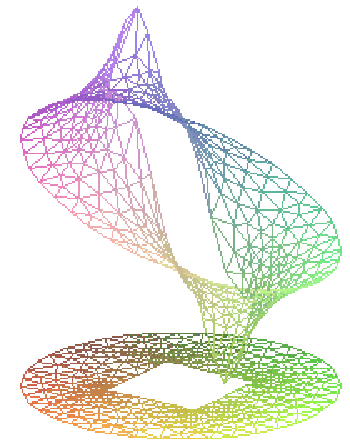
\includegraphics[height=7.0em, bb = 0 0 168 214]{images/img/logdim.ps}}  
  }

%%%%%%%%%%%%%%%%%%%%%%%%%%%%%%%%%%%%%%%%%%%%%%%%%%%%%%%%%%%%%%%%%%%%%%%%%%%%%%
%%% Now define the boxes that make up the poster
%%%---------------------------------------------------------------------------
%%% Each box has a name and can be placed absolutely or relatively.
%%% The only inconvenience is that you can only specify a relative position 
%%% towards an already declared box. So if you have a box attached to the 
%%% bottom, one to the top and a third one which should be in between, you 
%%% have to specify the top and bottom boxes before you specify the middle 
%%% box.
%%%%%%%%%%%%%%%%%%%%%%%%%%%%%%%%%%%%%%%%%%%%%%%%%%%%%%%%%%%%%%%%%%%%%%%%%%%%%%
    %
    % A coloured circle useful as a bullet with an adjustably strong filling
    \newcommand{\colouredcircle}{%
      \tikz{\useasboundingbox (-0.2em,-0.32em) rectangle(0.2em,0.32em); \draw[draw=black,fill=lightblue,line width=0.03em] (0,0) circle(0.18em);}}
%%%%%%%%%%%%%%%%%%%%%%%%%%%%%%%%%%%%%%%%%%%%%%%%%%%%%%%%%%%%%%%%%%%%%%%%%%%%%%
  \headerbox{Generality}{name=prev,column=0,span=6,row=0}{
  \noindent A {\emph{\bf cellular automata}} (CA) is a function $F\in \text{End}(Q^\ZZ)$ defined by $(N,f)$, where $N\subset \ZZ$ finite is called neighborhood, and
  $f:Q^{N}\to Q$ is such that $F(c)_i=f(c_{N+i})$. 
  \vspace{-0.75em}\\
  
  \noindent A reversible CA is  {\emph{\bf intrinsically universal}} if it can simulate any reversible CA. Durand-Lose (STACS 1997) shows that there exists a particioned 
  CA $\mathcal{U}$ which is intrinsically universal.
  }
%%%%%%%%%%%%%%%%%%%%%%%%%%%%%%%%%%%%%%%%%%%%%%%%%%%%%%%%%%%%%%%%%%%%%%%%%%%%%%
%%%%%%%%%%%%%%%%%%%%%%%%%%%%%%%%%%%%%%%%%%%%%%%%%%%%%%%%%%%%%%%%%%%%%%%%%%%%%%
  \headerbox{Number-conserving}{name=conser,column=0,row=0,below=prev,span=2}{
%%%%%%%%%%%%%%%%%%%%%%%%%%%%%%%%%%%%%%%%%%%%%%%%%%%%%%%%%%%%%%%%%%%%%%%%%%%%%%

\noindent We say that $F\in \text{End}(Q^\ZZ)$, with $Q=\{0,...,s-1\}$ is {\emph{\bf \green Number-Conserving}} (NCCA) if 
$\forall \alpha \in Q^\ZZ$ finite (i.e. $|\{\alpha_i:\alpha_i\not=0\}|<\infty$)
$$\sum_{i\in \ZZ}F(\alpha)_i=\sum_{i\in \ZZ}\alpha_i$$
 }

%%%%%%%%%%%%%%%%%%%%%%%%%%%%%%%%%%%%%%%%%%%%%%%%%%%%%%%%%%%%%%%%%%%%%%%%%%%%%%
  \headerbox{Example NCCA: Traffic rule}{name=ex_c,column=0,below=conser,span=2}{
%%%%%%%%%%%%%%%%%%%%%%%%%%%%%%%%%%%%%%%%%%%%%%%%%%%%%%%%%%%%%%%%%%%%%%%%%%%%%%
\begin{center}
\psscalebox{0.6 0.6}  %Change this value to rescale the drawing.
{
\hspace{-30pt}
\begin{pspicture}(0,0)(12.75,7.5)
\psframe[linecolor=black, linewidth=0.025, fillstyle=solid,fillcolor=red, dimen=outer](0.725,-0.025)(1.5,0.75)
\rput(1.1,0.35){ }
\psframe[linecolor=black, linewidth=0.025, fillstyle=solid,fillcolor=red, dimen=outer](1.475,-0.025)(2.25,0.75)
\rput(1.85,0.35){ }
\psframe[linecolor=black, linewidth=0.025, fillstyle=solid,fillcolor=red, dimen=outer](2.225,-0.025)(3,0.75)
\rput(2.6,0.35){ }
\psframe[linecolor=black, linewidth=0.025, fillstyle=solid,fillcolor=orange, dimen=outer](2.975,-0.025)(3.75,0.75)
\rput(3.35,0.35){$>$}
\psframe[linecolor=black, linewidth=0.025, fillstyle=solid,fillcolor=red, dimen=outer](3.725,-0.025)(4.5,0.75)
\rput(4.1,0.35){ }
\psframe[linecolor=black, linewidth=0.025, fillstyle=solid,fillcolor=red, dimen=outer](4.475,-0.025)(5.25,0.75)
\rput(4.85,0.35){ }
\psframe[linecolor=black, linewidth=0.025, fillstyle=solid,fillcolor=red, dimen=outer](5.225,-0.025)(6,0.75)
\rput(5.6,0.35){ }
\psframe[linecolor=black, linewidth=0.025, fillstyle=solid,fillcolor=orange, dimen=outer](5.975,-0.025)(6.75,0.75)
\rput(6.35,0.35){$>$}
\psframe[linecolor=black, linewidth=0.025, fillstyle=solid,fillcolor=orange, dimen=outer](6.725,-0.025)(7.5,0.75)
\rput(7.1,0.35){$>$}
\psframe[linecolor=black, linewidth=0.025, fillstyle=solid,fillcolor=orange, dimen=outer](7.475,-0.025)(8.25,0.75)
\rput(7.85,0.35){$>$}
\psframe[linecolor=black, linewidth=0.025, fillstyle=solid,fillcolor=orange, dimen=outer](8.225,-0.025)(9,0.75)
\rput(8.6,0.35){$>$}
\psframe[linecolor=black, linewidth=0.025, fillstyle=solid,fillcolor=orange, dimen=outer](8.975,-0.025)(9.75,0.75)
\rput(9.35,0.35){$>$}
\psframe[linecolor=black, linewidth=0.025, fillstyle=solid,fillcolor=red, dimen=outer](9.725,-0.025)(10.5,0.75)
\rput(10.1,0.35){ }
\psframe[linecolor=black, linewidth=0.025, fillstyle=solid,fillcolor=red, dimen=outer](10.475,-0.025)(11.25,0.75)
\rput(10.85,0.35){ }
\psframe[linecolor=black, linewidth=0.025, fillstyle=solid,fillcolor=red, dimen=outer](11.225,-0.025)(12,0.75)
\rput(11.6,0.35){ }
\psframe[linecolor=black, linewidth=0.025, fillstyle=solid,fillcolor=red, dimen=outer](11.975,-0.025)(12.75,0.75)
\rput(12.35,0.35){ }
\psframe[linecolor=black, linewidth=0.025, fillstyle=solid,fillcolor=red, dimen=outer](12.725,-0.025)(13.5,0.75)
\rput(13.1,0.35){ }
\psframe[linecolor=black, linewidth=0.025, fillstyle=solid,fillcolor=red, dimen=outer](0.725,0.725)(1.5,1.5)
\rput(1.1,1.1){ }
\psframe[linecolor=black, linewidth=0.025, fillstyle=solid,fillcolor=red, dimen=outer](1.475,0.725)(2.25,1.5)
\rput(1.85,1.1){ }
\psframe[linecolor=black, linewidth=0.025, fillstyle=solid,fillcolor=red, dimen=outer](2.225,0.725)(3,1.5)
\rput(2.6,1.1){ }
\psframe[linecolor=black, linewidth=0.025, fillstyle=solid,fillcolor=red, dimen=outer](2.975,0.725)(3.75,1.5)
\rput(3.35,1.1){ }
\psframe[linecolor=black, linewidth=0.025, fillstyle=solid,fillcolor=orange, dimen=outer](3.725,0.725)(4.5,1.5)
\rput(4.1,1.1){$>$}
\psframe[linecolor=black, linewidth=0.025, fillstyle=solid,fillcolor=red, dimen=outer](4.475,0.725)(5.25,1.5)
\rput(4.85,1.1){ }
\psframe[linecolor=black, linewidth=0.025, fillstyle=solid,fillcolor=red, dimen=outer](5.225,0.725)(6,1.5)
\rput(5.6,1.1){ }
\psframe[linecolor=black, linewidth=0.025, fillstyle=solid,fillcolor=orange, dimen=outer](5.975,0.725)(6.75,1.5)
\rput(6.35,1.1){$>$}
\psframe[linecolor=black, linewidth=0.025, fillstyle=solid,fillcolor=orange, dimen=outer](6.725,0.725)(7.5,1.5)
\rput(7.1,1.1){$>$}
\psframe[linecolor=black, linewidth=0.025, fillstyle=solid,fillcolor=orange, dimen=outer](7.475,0.725)(8.25,1.5)
\rput(7.85,1.1){$>$}
\psframe[linecolor=black, linewidth=0.025, fillstyle=solid,fillcolor=orange, dimen=outer](8.225,0.725)(9,1.5)
\rput(8.6,1.1){$>$}
\psframe[linecolor=black, linewidth=0.025, fillstyle=solid,fillcolor=red, dimen=outer](8.975,0.725)(9.75,1.5)
\rput(9.35,1.1){ }
\psframe[linecolor=black, linewidth=0.025, fillstyle=solid,fillcolor=orange, dimen=outer](9.725,0.725)(10.5,1.5)
\rput(10.1,1.1){$>$}
\psframe[linecolor=black, linewidth=0.025, fillstyle=solid,fillcolor=red, dimen=outer](10.475,0.725)(11.25,1.5)
\rput(10.85,1.1){ }
\psframe[linecolor=black, linewidth=0.025, fillstyle=solid,fillcolor=red, dimen=outer](11.225,0.725)(12,1.5)
\rput(11.6,1.1){ }
\psframe[linecolor=black, linewidth=0.025, fillstyle=solid,fillcolor=red, dimen=outer](11.975,0.725)(12.75,1.5)
\rput(12.35,1.1){ }
\psframe[linecolor=black, linewidth=0.025, fillstyle=solid,fillcolor=red, dimen=outer](12.725,0.725)(13.5,1.5)
\rput(13.1,1.1){ }
\psframe[linecolor=black, linewidth=0.025, fillstyle=solid,fillcolor=red, dimen=outer](0.725,1.475)(1.5,2.25)
\rput(1.1,1.85){ }
\psframe[linecolor=black, linewidth=0.025, fillstyle=solid,fillcolor=red, dimen=outer](1.475,1.475)(2.25,2.25)
\rput(1.85,1.85){ }
\psframe[linecolor=black, linewidth=0.025, fillstyle=solid,fillcolor=red, dimen=outer](2.225,1.475)(3,2.25)
\rput(2.6,1.85){ }
\psframe[linecolor=black, linewidth=0.025, fillstyle=solid,fillcolor=red, dimen=outer](2.975,1.475)(3.75,2.25)
\rput(3.35,1.85){ }
\psframe[linecolor=black, linewidth=0.025, fillstyle=solid,fillcolor=red, dimen=outer](3.725,1.475)(4.5,2.25)
\rput(4.1,1.85){ }
\psframe[linecolor=black, linewidth=0.025, fillstyle=solid,fillcolor=orange, dimen=outer](4.475,1.475)(5.25,2.25)
\rput(4.85,1.85){$>$}
\psframe[linecolor=black, linewidth=0.025, fillstyle=solid,fillcolor=red, dimen=outer](5.225,1.475)(6,2.25)
\rput(5.6,1.85){ }
\psframe[linecolor=black, linewidth=0.025, fillstyle=solid,fillcolor=orange, dimen=outer](5.975,1.475)(6.75,2.25)
\rput(6.35,1.85){$>$}
\psframe[linecolor=black, linewidth=0.025, fillstyle=solid,fillcolor=orange, dimen=outer](6.725,1.475)(7.5,2.25)
\rput(7.1,1.85){$>$}
\psframe[linecolor=black, linewidth=0.025, fillstyle=solid,fillcolor=orange, dimen=outer](7.475,1.475)(8.25,2.25)
\rput(7.85,1.85){$>$}
\psframe[linecolor=black, linewidth=0.025, fillstyle=solid,fillcolor=red, dimen=outer](8.225,1.475)(9,2.25)
\rput(8.6,1.85){ }
\psframe[linecolor=black, linewidth=0.025, fillstyle=solid,fillcolor=orange, dimen=outer](8.975,1.475)(9.75,2.25)
\rput(9.35,1.85){$>$}
\psframe[linecolor=black, linewidth=0.025, fillstyle=solid,fillcolor=red, dimen=outer](9.725,1.475)(10.5,2.25)
\rput(10.1,1.85){ }
\psframe[linecolor=black, linewidth=0.025, fillstyle=solid,fillcolor=orange, dimen=outer](10.475,1.475)(11.25,2.25)
\rput(10.85,1.85){$>$}
\psframe[linecolor=black, linewidth=0.025, fillstyle=solid,fillcolor=red, dimen=outer](11.225,1.475)(12,2.25)
\rput(11.6,1.85){ }
\psframe[linecolor=black, linewidth=0.025, fillstyle=solid,fillcolor=red, dimen=outer](11.975,1.475)(12.75,2.25)
\rput(12.35,1.85){ }
\psframe[linecolor=black, linewidth=0.025, fillstyle=solid,fillcolor=red, dimen=outer](12.725,1.475)(13.5,2.25)
\rput(13.1,1.85){ }
\psframe[linecolor=black, linewidth=0.025, fillstyle=solid,fillcolor=red, dimen=outer](0.725,2.225)(1.5,3)
\rput(1.1,2.6){ }
\psframe[linecolor=black, linewidth=0.025, fillstyle=solid,fillcolor=red, dimen=outer](1.475,2.225)(2.25,3)
\rput(1.85,2.6){ }
\psframe[linecolor=black, linewidth=0.025, fillstyle=solid,fillcolor=red, dimen=outer](2.225,2.225)(3,3)
\rput(2.6,2.6){ }
\psframe[linecolor=black, linewidth=0.025, fillstyle=solid,fillcolor=red, dimen=outer](2.975,2.225)(3.75,3)
\rput(3.35,2.6){ }
\psframe[linecolor=black, linewidth=0.025, fillstyle=solid,fillcolor=red, dimen=outer](3.725,2.225)(4.5,3)
\rput(4.1,2.6){ }
\psframe[linecolor=black, linewidth=0.025, fillstyle=solid,fillcolor=red, dimen=outer](4.475,2.225)(5.25,3)
\rput(4.85,2.6){ }
\psframe[linecolor=black, linewidth=0.025, fillstyle=solid,fillcolor=orange, dimen=outer](5.225,2.225)(6,3)
\rput(5.6,2.6){$>$}
\psframe[linecolor=black, linewidth=0.025, fillstyle=solid,fillcolor=orange, dimen=outer](5.975,2.225)(6.75,3)
\rput(6.35,2.6){$>$}
\psframe[linecolor=black, linewidth=0.025, fillstyle=solid,fillcolor=orange, dimen=outer](6.725,2.225)(7.5,3)
\rput(7.1,2.6){$>$}
\psframe[linecolor=black, linewidth=0.025, fillstyle=solid,fillcolor=red, dimen=outer](7.475,2.225)(8.25,3)
\rput(7.85,2.6){ }
\psframe[linecolor=black, linewidth=0.025, fillstyle=solid,fillcolor=orange, dimen=outer](8.225,2.225)(9,3)
\rput(8.6,2.6){$>$}
\psframe[linecolor=black, linewidth=0.025, fillstyle=solid,fillcolor=red, dimen=outer](8.975,2.225)(9.75,3)
\rput(9.35,2.6){ }
\psframe[linecolor=black, linewidth=0.025, fillstyle=solid,fillcolor=orange, dimen=outer](9.725,2.225)(10.5,3)
\rput(10.1,2.6){$>$}
\psframe[linecolor=black, linewidth=0.025, fillstyle=solid,fillcolor=red, dimen=outer](10.475,2.225)(11.25,3)
\rput(10.85,2.6){ }
\psframe[linecolor=black, linewidth=0.025, fillstyle=solid,fillcolor=orange, dimen=outer](11.225,2.225)(12,3)
\rput(11.6,2.6){$>$}
\psframe[linecolor=black, linewidth=0.025, fillstyle=solid,fillcolor=red, dimen=outer](11.975,2.225)(12.75,3)
\rput(12.35,2.6){ }
\psframe[linecolor=black, linewidth=0.025, fillstyle=solid,fillcolor=red, dimen=outer](12.725,2.225)(13.5,3)
\rput(13.1,2.6){ }
\psframe[linecolor=black, linewidth=0.025, fillstyle=solid,fillcolor=red, dimen=outer](0.725,2.975)(1.5,3.75)
\rput(1.1,3.35){ }
\psframe[linecolor=black, linewidth=0.025, fillstyle=solid,fillcolor=red, dimen=outer](1.475,2.975)(2.25,3.75)
\rput(1.85,3.35){ }
\psframe[linecolor=black, linewidth=0.025, fillstyle=solid,fillcolor=red, dimen=outer](2.225,2.975)(3,3.75)
\rput(2.6,3.35){ }
\psframe[linecolor=black, linewidth=0.025, fillstyle=solid,fillcolor=red, dimen=outer](2.975,2.975)(3.75,3.75)
\rput(3.35,3.35){ }
\psframe[linecolor=black, linewidth=0.025, fillstyle=solid,fillcolor=red, dimen=outer](3.725,2.975)(4.5,3.75)
\rput(4.1,3.35){ }
\psframe[linecolor=black, linewidth=0.025, fillstyle=solid,fillcolor=red, dimen=outer](4.475,2.975)(5.25,3.75)
\rput(4.85,3.35){ }
\psframe[linecolor=black, linewidth=0.025, fillstyle=solid,fillcolor=orange, dimen=outer](5.225,2.975)(6,3.75)
\rput(5.6,3.35){$>$}
\psframe[linecolor=black, linewidth=0.025, fillstyle=solid,fillcolor=orange, dimen=outer](5.975,2.975)(6.75,3.75)
\rput(6.35,3.35){$>$}
\psframe[linecolor=black, linewidth=0.025, fillstyle=solid,fillcolor=red, dimen=outer](6.725,2.975)(7.5,3.75)
\rput(7.1,3.35){ }
\psframe[linecolor=black, linewidth=0.025, fillstyle=solid,fillcolor=orange, dimen=outer](7.475,2.975)(8.25,3.75)
\rput(7.85,3.35){$>$}
\psframe[linecolor=black, linewidth=0.025, fillstyle=solid,fillcolor=red, dimen=outer](8.225,2.975)(9,3.75)
\rput(8.6,3.35){ }
\psframe[linecolor=black, linewidth=0.025, fillstyle=solid,fillcolor=orange, dimen=outer](8.975,2.975)(9.75,3.75)
\rput(9.35,3.35){$>$}
\psframe[linecolor=black, linewidth=0.025, fillstyle=solid,fillcolor=red, dimen=outer](9.725,2.975)(10.5,3.75)
\rput(10.1,3.35){ }
\psframe[linecolor=black, linewidth=0.025, fillstyle=solid,fillcolor=orange, dimen=outer](10.475,2.975)(11.25,3.75)
\rput(10.85,3.35){$>$}
\psframe[linecolor=black, linewidth=0.025, fillstyle=solid,fillcolor=red, dimen=outer](11.225,2.975)(12,3.75)
\rput(11.6,3.35){ }
\psframe[linecolor=black, linewidth=0.025, fillstyle=solid,fillcolor=orange, dimen=outer](11.975,2.975)(12.75,3.75)
\rput(12.35,3.35){$>$}
\psframe[linecolor=black, linewidth=0.025, fillstyle=solid,fillcolor=red, dimen=outer](12.725,2.975)(13.5,3.75)
\rput(13.1,3.35){ }
\psframe[linecolor=black, linewidth=0.025, fillstyle=solid,fillcolor=red, dimen=outer](0.725,3.725)(1.5,4.5)
\rput(1.1,4.1){ }
\psframe[linecolor=black, linewidth=0.025, fillstyle=solid,fillcolor=red, dimen=outer](1.475,3.725)(2.25,4.5)
\rput(1.85,4.1){ }
\psframe[linecolor=black, linewidth=0.025, fillstyle=solid,fillcolor=red, dimen=outer](2.225,3.725)(3,4.5)
\rput(2.6,4.1){ }
\psframe[linecolor=black, linewidth=0.025, fillstyle=solid,fillcolor=red, dimen=outer](2.975,3.725)(3.75,4.5)
\rput(3.35,4.1){ }
\psframe[linecolor=black, linewidth=0.025, fillstyle=solid,fillcolor=red, dimen=outer](3.725,3.725)(4.5,4.5)
\rput(4.1,4.1){ }
\psframe[linecolor=black, linewidth=0.025, fillstyle=solid,fillcolor=red, dimen=outer](4.475,3.725)(5.25,4.5)
\rput(4.85,4.1){ }
\psframe[linecolor=black, linewidth=0.025, fillstyle=solid,fillcolor=orange, dimen=outer](5.225,3.725)(6,4.5)
\rput(5.6,4.1){$>$}
\psframe[linecolor=black, linewidth=0.025, fillstyle=solid,fillcolor=red, dimen=outer](5.975,3.725)(6.75,4.5)
\rput(6.35,4.1){ }
\psframe[linecolor=black, linewidth=0.025, fillstyle=solid,fillcolor=orange, dimen=outer](6.725,3.725)(7.5,4.5)
\rput(7.1,4.1){$>$}
\psframe[linecolor=black, linewidth=0.025, fillstyle=solid,fillcolor=red, dimen=outer](7.475,3.725)(8.25,4.5)
\rput(7.85,4.1){ }
\psframe[linecolor=black, linewidth=0.025, fillstyle=solid,fillcolor=orange, dimen=outer](8.225,3.725)(9,4.5)
\rput(8.6,4.1){$>$}
\psframe[linecolor=black, linewidth=0.025, fillstyle=solid,fillcolor=red, dimen=outer](8.975,3.725)(9.75,4.5)
\rput(9.35,4.1){ }
\psframe[linecolor=black, linewidth=0.025, fillstyle=solid,fillcolor=orange, dimen=outer](9.725,3.725)(10.5,4.5)
\rput(10.1,4.1){$>$}
\psframe[linecolor=black, linewidth=0.025, fillstyle=solid,fillcolor=red, dimen=outer](10.475,3.725)(11.25,4.5)
\rput(10.85,4.1){ }
\psframe[linecolor=black, linewidth=0.025, fillstyle=solid,fillcolor=orange, dimen=outer](11.225,3.725)(12,4.5)
\rput(11.6,4.1){$>$}
\psframe[linecolor=black, linewidth=0.025, fillstyle=solid,fillcolor=red, dimen=outer](11.975,3.725)(12.75,4.5)
\rput(12.35,4.1){ }
\psframe[linecolor=black, linewidth=0.025, fillstyle=solid,fillcolor=orange, dimen=outer](12.725,3.725)(13.5,4.5)
\rput(13.1,4.1){$>$}
\psframe[linecolor=black, linewidth=0.025, fillstyle=solid,fillcolor=red, dimen=outer](0.725,4.475)(1.5,5.25)
\rput(1.1,4.85){ }
\psframe[linecolor=black, linewidth=0.025, fillstyle=solid,fillcolor=red, dimen=outer](1.475,4.475)(2.25,5.25)
\rput(1.85,4.85){ }
\psframe[linecolor=black, linewidth=0.025, fillstyle=solid,fillcolor=red, dimen=outer](2.225,4.475)(3,5.25)
\rput(2.6,4.85){ }
\psframe[linecolor=black, linewidth=0.025, fillstyle=solid,fillcolor=red, dimen=outer](2.975,4.475)(3.75,5.25)
\rput(3.35,4.85){ }
\psframe[linecolor=black, linewidth=0.025, fillstyle=solid,fillcolor=red, dimen=outer](3.725,4.475)(4.5,5.25)
\rput(4.1,4.85){ }
\psframe[linecolor=black, linewidth=0.025, fillstyle=solid,fillcolor=red, dimen=outer](4.475,4.475)(5.25,5.25)
\rput(4.85,4.85){ }
\psframe[linecolor=black, linewidth=0.025, fillstyle=solid,fillcolor=red, dimen=outer](5.225,4.475)(6,5.25)
\rput(5.6,4.85){ }
\psframe[linecolor=black, linewidth=0.025, fillstyle=solid,fillcolor=orange, dimen=outer](5.975,4.475)(6.75,5.25)
\rput(6.35,4.85){$>$}
\psframe[linecolor=black, linewidth=0.025, fillstyle=solid,fillcolor=red, dimen=outer](6.725,4.475)(7.5,5.25)
\rput(7.1,4.85){ }
\psframe[linecolor=black, linewidth=0.025, fillstyle=solid,fillcolor=orange, dimen=outer](7.475,4.475)(8.25,5.25)
\rput(7.85,4.85){$>$}
\psframe[linecolor=black, linewidth=0.025, fillstyle=solid,fillcolor=red, dimen=outer](8.225,4.475)(9,5.25)
\rput(8.6,4.85){ }
\psframe[linecolor=black, linewidth=0.025, fillstyle=solid,fillcolor=orange, dimen=outer](8.975,4.475)(9.75,5.25)
\rput(9.35,4.85){$>$}
\psframe[linecolor=black, linewidth=0.025, fillstyle=solid,fillcolor=red, dimen=outer](9.725,4.475)(10.5,5.25)
\rput(10.1,4.85){ }
\psframe[linecolor=black, linewidth=0.025, fillstyle=solid,fillcolor=orange, dimen=outer](10.475,4.475)(11.25,5.25)
\rput(10.85,4.85){$>$}
\psframe[linecolor=black, linewidth=0.025, fillstyle=solid,fillcolor=red, dimen=outer](11.225,4.475)(12,5.25)
\rput(11.6,4.85){ }
\psframe[linecolor=black, linewidth=0.025, fillstyle=solid,fillcolor=orange, dimen=outer](11.975,4.475)(12.75,5.25)
\rput(12.35,4.85){$>$}
\psframe[linecolor=black, linewidth=0.025, fillstyle=solid,fillcolor=red, dimen=outer](12.725,4.475)(13.5,5.25)
\rput(13.1,4.85){ }
\psframe[linecolor=black, linewidth=0.025, fillstyle=solid,fillcolor=red, dimen=outer](0.725,5.225)(1.5,6)
\rput(1.1,5.6){ }
\psframe[linecolor=black, linewidth=0.025, fillstyle=solid,fillcolor=red, dimen=outer](1.475,5.225)(2.25,6)
\rput(1.85,5.6){ }
\psframe[linecolor=black, linewidth=0.025, fillstyle=solid,fillcolor=red, dimen=outer](2.225,5.225)(3,6)
\rput(2.6,5.6){ }
\psframe[linecolor=black, linewidth=0.025, fillstyle=solid,fillcolor=red, dimen=outer](2.975,5.225)(3.75,6)
\rput(3.35,5.6){ }
\psframe[linecolor=black, linewidth=0.025, fillstyle=solid,fillcolor=red, dimen=outer](3.725,5.225)(4.5,6)
\rput(4.1,5.6){ }
\psframe[linecolor=black, linewidth=0.025, fillstyle=solid,fillcolor=red, dimen=outer](4.475,5.225)(5.25,6)
\rput(4.85,5.6){ }
\psframe[linecolor=black, linewidth=0.025, fillstyle=solid,fillcolor=red, dimen=outer](5.225,5.225)(6,6)
\rput(5.6,5.6){ }
\psframe[linecolor=black, linewidth=0.025, fillstyle=solid,fillcolor=red, dimen=outer](5.975,5.225)(6.75,6)
\rput(6.35,5.6){ }
\psframe[linecolor=black, linewidth=0.025, fillstyle=solid,fillcolor=orange, dimen=outer](6.725,5.225)(7.5,6)
\rput(7.1,5.6){$>$}
\psframe[linecolor=black, linewidth=0.025, fillstyle=solid,fillcolor=red, dimen=outer](7.475,5.225)(8.25,6)
\rput(7.85,5.6){ }
\psframe[linecolor=black, linewidth=0.025, fillstyle=solid,fillcolor=orange, dimen=outer](8.225,5.225)(9,6)
\rput(8.6,5.6){$>$}
\psframe[linecolor=black, linewidth=0.025, fillstyle=solid,fillcolor=red, dimen=outer](8.975,5.225)(9.75,6)
\rput(9.35,5.6){ }
\psframe[linecolor=black, linewidth=0.025, fillstyle=solid,fillcolor=orange, dimen=outer](9.725,5.225)(10.5,6)
\rput(10.1,5.6){$>$}
\psframe[linecolor=black, linewidth=0.025, fillstyle=solid,fillcolor=red, dimen=outer](10.475,5.225)(11.25,6)
\rput(10.85,5.6){ }
\psframe[linecolor=black, linewidth=0.025, fillstyle=solid,fillcolor=orange, dimen=outer](11.225,5.225)(12,6)
\rput(11.6,5.6){$>$}
\psframe[linecolor=black, linewidth=0.025, fillstyle=solid,fillcolor=red, dimen=outer](11.975,5.225)(12.75,6)
\rput(12.35,5.6){ }
\psframe[linecolor=black, linewidth=0.025, fillstyle=solid,fillcolor=orange, dimen=outer](12.725,5.225)(13.5,6)
\rput(13.1,5.6){$>$}
\psframe[linecolor=black, linewidth=0.025, fillstyle=solid,fillcolor=red, dimen=outer](0.725,5.975)(1.5,6.75)
\rput(1.1,6.35){ }
\psframe[linecolor=black, linewidth=0.025, fillstyle=solid,fillcolor=red, dimen=outer](1.475,5.975)(2.25,6.75)
\rput(1.85,6.35){ }
\psframe[linecolor=black, linewidth=0.025, fillstyle=solid,fillcolor=red, dimen=outer](2.225,5.975)(3,6.75)
\rput(2.6,6.35){ }
\psframe[linecolor=black, linewidth=0.025, fillstyle=solid,fillcolor=red, dimen=outer](2.975,5.975)(3.75,6.75)
\rput(3.35,6.35){ }
\psframe[linecolor=black, linewidth=0.025, fillstyle=solid,fillcolor=red, dimen=outer](3.725,5.975)(4.5,6.75)
\rput(4.1,6.35){ }
\psframe[linecolor=black, linewidth=0.025, fillstyle=solid,fillcolor=red, dimen=outer](4.475,5.975)(5.25,6.75)
\rput(4.85,6.35){ }
\psframe[linecolor=black, linewidth=0.025, fillstyle=solid,fillcolor=red, dimen=outer](5.225,5.975)(6,6.75)
\rput(5.6,6.35){ }
\psframe[linecolor=black, linewidth=0.025, fillstyle=solid,fillcolor=red, dimen=outer](5.975,5.975)(6.75,6.75)
\rput(6.35,6.35){ }
\psframe[linecolor=black, linewidth=0.025, fillstyle=solid,fillcolor=red, dimen=outer](6.725,5.975)(7.5,6.75)
\rput(7.1,6.35){ }
\psframe[linecolor=black, linewidth=0.025, fillstyle=solid,fillcolor=orange, dimen=outer](7.475,5.975)(8.25,6.75)
\rput(7.85,6.35){$>$}
\psframe[linecolor=black, linewidth=0.025, fillstyle=solid,fillcolor=red, dimen=outer](8.225,5.975)(9,6.75)
\rput(8.6,6.35){ }
\psframe[linecolor=black, linewidth=0.025, fillstyle=solid,fillcolor=orange, dimen=outer](8.975,5.975)(9.75,6.75)
\rput(9.35,6.35){$>$}
\psframe[linecolor=black, linewidth=0.025, fillstyle=solid,fillcolor=red, dimen=outer](9.725,5.975)(10.5,6.75)
\rput(10.1,6.35){ }
\psframe[linecolor=black, linewidth=0.025, fillstyle=solid,fillcolor=orange, dimen=outer](10.475,5.975)(11.25,6.75)
\rput(10.85,6.35){$>$}
\psframe[linecolor=black, linewidth=0.025, fillstyle=solid,fillcolor=red, dimen=outer](11.225,5.975)(12,6.75)
\rput(11.6,6.35){ }
\psframe[linecolor=black, linewidth=0.025, fillstyle=solid,fillcolor=orange, dimen=outer](11.975,5.975)(12.75,6.75)
\rput(12.35,6.35){$>$}
\psframe[linecolor=black, linewidth=0.025, fillstyle=solid,fillcolor=red, dimen=outer](12.725,5.975)(13.5,6.75)
\rput(13.1,6.35){ }
\psframe[linecolor=black, linewidth=0.025, fillstyle=solid,fillcolor=red, dimen=outer](0.725,6.725)(1.5,7.5)
\rput(1.1,7.1){ }
\psframe[linecolor=black, linewidth=0.025, fillstyle=solid,fillcolor=red, dimen=outer](1.475,6.725)(2.25,7.5)
\rput(1.85,7.1){ }
\psframe[linecolor=black, linewidth=0.025, fillstyle=solid,fillcolor=red, dimen=outer](2.225,6.725)(3,7.5)
\rput(2.6,7.1){ }
\psframe[linecolor=black, linewidth=0.025, fillstyle=solid,fillcolor=red, dimen=outer](2.975,6.725)(3.75,7.5)
\rput(3.35,7.1){ }
\psframe[linecolor=black, linewidth=0.025, fillstyle=solid,fillcolor=red, dimen=outer](3.725,6.725)(4.5,7.5)
\rput(4.1,7.1){ }
\psframe[linecolor=black, linewidth=0.025, fillstyle=solid,fillcolor=red, dimen=outer](4.475,6.725)(5.25,7.5)
\rput(4.85,7.1){ }
\psframe[linecolor=black, linewidth=0.025, fillstyle=solid,fillcolor=red, dimen=outer](5.225,6.725)(6,7.5)
\rput(5.6,7.1){ }
\psframe[linecolor=black, linewidth=0.025, fillstyle=solid,fillcolor=red, dimen=outer](5.975,6.725)(6.75,7.5)
\rput(6.35,7.1){ }
\psframe[linecolor=black, linewidth=0.025, fillstyle=solid,fillcolor=red, dimen=outer](6.725,6.725)(7.5,7.5)
\rput(7.1,7.1){ }
\psframe[linecolor=black, linewidth=0.025, fillstyle=solid,fillcolor=red, dimen=outer](7.475,6.725)(8.25,7.5)
\rput(7.85,7.1){ }
\psframe[linecolor=black, linewidth=0.025, fillstyle=solid,fillcolor=orange, dimen=outer](8.225,6.725)(9,7.5)
\rput(8.6,7.1){$>$}
\psframe[linecolor=black, linewidth=0.025, fillstyle=solid,fillcolor=red, dimen=outer](8.975,6.725)(9.75,7.5)
\rput(9.35,7.1){ }
\psframe[linecolor=black, linewidth=0.025, fillstyle=solid,fillcolor=orange, dimen=outer](9.725,6.725)(10.5,7.5)
\rput(10.1,7.1){$>$}
\psframe[linecolor=black, linewidth=0.025, fillstyle=solid,fillcolor=red, dimen=outer](10.475,6.725)(11.25,7.5)
\rput(10.85,7.1){ }
\psframe[linecolor=black, linewidth=0.025, fillstyle=solid,fillcolor=orange, dimen=outer](11.225,6.725)(12,7.5)
\rput(11.6,7.1){$>$}
\psframe[linecolor=black, linewidth=0.025, fillstyle=solid,fillcolor=red, dimen=outer](11.975,6.725)(12.75,7.5)
\rput(12.35,7.1){ }
\psframe[linecolor=black, linewidth=0.025, fillstyle=solid,fillcolor=orange, dimen=outer](12.725,6.725)(13.5,7.5)
\rput(13.1,7.1){$>$}
\end{pspicture}
}
\end{center}
  }
%%%%%%%%%%%%%%%%%%%%%%%%%%%%%%%%%%%%%%%%%%%%%%%%%%%%%%%%%%%%%%%%%%%%%%%%%%%%%%
  \headerbox{Moreira THEOR COMPUT SCI 2003}{name=sim_more,column=0,below=ex_c,span=4}{
%%%%%%%%%%%%%%%%%%%%%%%%%%%%%%%%%%%%%%%%%%%%%%%%%%%%%%%%%%%%%%%%%%%%%%%%%%%%%%
 \noindent Given a CA $F$ with $s$ states and neighborhood with size $n$, then exists a NCCA $G$ with states 
 $\{-s,... s\}$ and neighborhood with size $2n$ such that the next diagram commute 
%  $$A\preccurlyeq B$$ 
\begin{center}
\psscalebox{0.8 0.8} % Change this value to rescale the drawing.
{
\begin{pspicture}(0,-1.4509524)(17.571428,1.4509524)
\rput(3.647619,1.0690477){$\alpha_i$ }
\psline[linecolor=black, linewidth=0.04, arrowsize=0.05291666666666668cm 2.0,arrowlength=1.4,arrowinset=0.0]{->}(3.687619,0.5709525)(3.687619,-0.70904756)
\rput[bl](8.527619,1.2109524){$F$}
\psline[linecolor=black, linewidth=0.04, arrowsize=0.05291666666666668cm 2.0,arrowlength=1.4,arrowinset=0.0]{->}(7.847619,0.9309524)(9.727619,0.9309524)
\rput[bl](3.2476192,-0.06904755){$\varphi$ }
\rput(5.047619,1.0690477){$\alpha_{i+1}$ }
\rput(6.447619,1.0690477){$\alpha_{i+1}$ }
\rput(2.2476192,1.0690477){$\alpha_{i-1}$ }
\rput(1.0476191,1.0690477){$\alpha_{i-2}$ }
\rput(2.2476192,-1.1570238){$-\alpha_{i-1}$ }
\rput(3.647619,-1.1570238){$\alpha_{i}$ }
\rput(5.047619,-1.1570238){$-\alpha_{i}$ }
\rput(1.0476191,-1.1570238){$\alpha_{i-1}$ }
\rput(6.447619,-1.1570238){$\alpha_{i+1}$ }
\psline[linecolor=black, linewidth=0.04](0.21904762,-0.8309523)(0.21904762,-1.4297234)
\psline[linecolor=black, linewidth=0.04](0.0,-1.4309523)(7.3714285,-1.4309523)
\psline[linecolor=black, linewidth=0.04](1.6190476,-0.8309523)(1.6190476,-1.4297234)
\psline[linecolor=black, linewidth=0.04](5.8190475,-0.8309523)(5.8190475,-1.4297234)
\psline[linecolor=black, linewidth=0.04](7.2190475,-0.8309523)(7.2190475,-1.4297234)
\psline[linecolor=black, linewidth=0.04](4.419048,-0.8309523)(4.419048,-1.4297234)
\psline[linecolor=black, linewidth=0.04](3.0190477,-0.8309523)(3.0190477,-1.4297234)
\psline[linecolor=black, linewidth=0.04](0.0,-0.8309523)(7.3714285,-0.8309523)
\psline[linecolor=black, linewidth=0.04](0.21904762,1.3690476)(0.21904762,0.77027655)
\psline[linecolor=black, linewidth=0.04](0.0,0.7690477)(7.3714285,0.7690477)
\psline[linecolor=black, linewidth=0.04](1.6190476,1.3690476)(1.6190476,0.77027655)
\psline[linecolor=black, linewidth=0.04](5.8190475,1.3690476)(5.8190475,0.77027655)
\psline[linecolor=black, linewidth=0.04](7.2190475,1.3690476)(7.2190475,0.77027655)
\psline[linecolor=black, linewidth=0.04](4.419048,1.3690476)(4.419048,0.77027655)
\psline[linecolor=black, linewidth=0.04](3.0190477,1.3690476)(3.0190477,0.77027655)
\psline[linecolor=black, linewidth=0.04](0.0,1.3690476)(7.3714285,1.3690476)
\rput(12.447619,-1.1309525){$\minus F(\alpha)_{i\minus1}$ }
\rput(13.847619,-1.1309525){$F(\alpha)_{i}$ }
\rput(15.247619,-1.1309525){$\minus F(\alpha)_{i}$ }
\rput(11.119047,-1.1309525){$F(\alpha)_{i-1}$ }
\rput(16.64762,-1.1309525){$F(\alpha)_{i+1}$ }
\psline[linecolor=black, linewidth=0.04](10.2,-0.8309523)(17.571428,-0.8309523)
\psline[linecolor=black, linewidth=0.04](16.019047,-0.8309523)(16.019047,-1.4297234)
\psline[linecolor=black, linewidth=0.04](17.419048,-0.8309523)(17.419048,-1.4297234)
\psline[linecolor=black, linewidth=0.04](14.619047,-0.8309523)(14.619047,-1.4297234)
\psline[linecolor=black, linewidth=0.04](13.219048,-0.8309523)(13.219048,-1.4297234)
\psline[linecolor=black, linewidth=0.04](11.819048,-0.8309523)(11.819048,-1.4297234)
\psline[linecolor=black, linewidth=0.04](10.419047,-0.8309523)(10.419047,-1.4297234)
\psline[linecolor=black, linewidth=0.04](10.2,-1.4309523)(17.571428,-1.4309523)
\psline[linecolor=black, linewidth=0.04](10.419047,1.3690476)(10.419047,0.77027655)
\psline[linecolor=black, linewidth=0.04](10.2,0.7690477)(17.571428,0.7690477)
\psline[linecolor=black, linewidth=0.04](11.819048,1.3690476)(11.819048,0.77027655)
\psline[linecolor=black, linewidth=0.04](16.019047,1.3690476)(16.019047,0.77027655)
\psline[linecolor=black, linewidth=0.04](17.419048,1.3690476)(17.419048,0.77027655)
\psline[linecolor=black, linewidth=0.04](14.619047,1.3690476)(14.619047,0.77027655)
\psline[linecolor=black, linewidth=0.04](13.219048,1.3690476)(13.219048,0.77027655)
\psline[linecolor=black, linewidth=0.04](10.2,1.3690476)(17.571428,1.3690476)
\rput(13.847619,1.0690476){$F(\alpha)_{i}$ }
\rput(15.247619,1.0690476){$F(\alpha)_{i+1}$ }
\rput(16.64762,1.0690476){$F(\alpha)_{i+2}$ }
\rput(12.447619,1.0690476){$F(\alpha)_{i-1}$ }
\rput(11.047619,1.0690476){$F(\alpha)_{i-2}$ }
\psline[linecolor=black, linewidth=0.04, arrowsize=0.05291666666666668cm 2.0,arrowlength=1.4,arrowinset=0.0]{->}(13.887619,0.5709525)(13.887619,-0.70904756)
\rput[bl](13.447619,-0.06904755){$\varphi$ }
\rput[bl](8.527619,-0.78904754){$G$}
\psline[linecolor=black, linewidth=0.04, arrowsize=0.05291666666666668cm 2.0,arrowlength=1.4,arrowinset=0.0]{->}(7.847619,-1.0690476)(9.727619,-1.0690476)
\end{pspicture}
}
\end{center}
  {\bf Problem:} In general  $G$ is not reversible, even if  $F$ does.
 }
%%%%%%%%%%%%%%%%%%%%%%%%%%%%%%%%%%%%%%%%%%%%%%%%%%%%%%%%%%%%%%%%%%%%%%%%%%%%%%
\headerbox{Reversibility}{name=rev,column=2,row=0,below=prev,span=2}{
  %%%%%%%%%%%%%%%%%%%%%%%%%%%%%%%%%%%%%%%%%%%%%%%%%%%%%%%%%%%%%%%%%%%%%%%%%%%%%%
 \noindent We say that a CA $F$ is {\emph{ \bf \red reversible}} (RCA) if there exists $F^{-1}$ and it is a CA .

}
%%%%%%%%%%%%%%%%%%%%%%%%%%%%%%%%%%%%%%%%%%%%%%%%%%%%%%%%%%%%%%%%%%%%%%%%%%%%%%
  \headerbox{Example RCA}{name=ex_r,column=2,below=rev,span=2}{
%%%%%%%%%%%%%%%%%%%%%%%%%%%%%%%%%%%%%%%%%%%%%%%%%%%%%%%%%%%%%%%%%%%%%%%%%%%%%%
\noindent
\begin{center}
\psscalebox{0.5 0.5}  %Change this value to rescale the drawing.
{
\hspace{-30pt}
\begin{pspicture}(0,0)(9.75,12)
\psframe[linecolor=black, linewidth=0.025, fillstyle=solid,fillcolor=white, dimen=outer](0.725,-0.025)(1.5,0.75)
\rput(1.1,0.35){ }
\psframe[linecolor=black, linewidth=0.025, fillstyle=solid,fillcolor=white, dimen=outer](1.475,-0.025)(2.25,0.75)
\rput(1.85,0.35){ }
\psframe[linecolor=black, linewidth=0.025, fillstyle=solid,fillcolor=blue, dimen=outer](2.225,-0.025)(3,0.75)
\rput(2.6,0.35){ }
\psframe[linecolor=black, linewidth=0.025, fillstyle=solid,fillcolor=white, dimen=outer](2.975,-0.025)(3.75,0.75)
\rput(3.35,0.35){ }
\psframe[linecolor=black, linewidth=0.025, fillstyle=solid,fillcolor=white, dimen=outer](3.725,-0.025)(4.5,0.75)
\rput(4.1,0.35){ }
\psframe[linecolor=black, linewidth=0.025, fillstyle=solid,fillcolor=orange, dimen=outer](4.475,-0.025)(5.25,0.75)
\rput(4.85,0.35){$>$}
\psframe[linecolor=black, linewidth=0.025, fillstyle=solid,fillcolor=white, dimen=outer](5.225,-0.025)(6,0.75)
\rput(5.6,0.35){ }
\psframe[linecolor=black, linewidth=0.025, fillstyle=solid,fillcolor=white, dimen=outer](5.975,-0.025)(6.75,0.75)
\rput(6.35,0.35){ }
\psframe[linecolor=black, linewidth=0.025, fillstyle=solid,fillcolor=white, dimen=outer](6.725,-0.025)(7.5,0.75)
\rput(7.1,0.35){ }
\psframe[linecolor=black, linewidth=0.025, fillstyle=solid,fillcolor=white, dimen=outer](7.475,-0.025)(8.25,0.75)
\rput(7.85,0.35){ }
\psframe[linecolor=black, linewidth=0.025, fillstyle=solid,fillcolor=white, dimen=outer](8.225,-0.025)(9,0.75)
\rput(8.6,0.35){ }
\psframe[linecolor=black, linewidth=0.025, fillstyle=solid,fillcolor=blue, dimen=outer](8.975,-0.025)(9.75,0.75)
\rput(9.35,0.35){ }
\psframe[linecolor=black, linewidth=0.025, fillstyle=solid,fillcolor=white, dimen=outer](9.725,-0.025)(10.5,0.75)
\rput(10.1,0.35){ }
\psframe[linecolor=black, linewidth=0.025, fillstyle=solid,fillcolor=white, dimen=outer](0.725,0.725)(1.5,1.5)
\rput(1.1,1.1){ }
\psframe[linecolor=black, linewidth=0.025, fillstyle=solid,fillcolor=white, dimen=outer](1.475,0.725)(2.25,1.5)
\rput(1.85,1.1){ }
\psframe[linecolor=black, linewidth=0.025, fillstyle=solid,fillcolor=blue, dimen=outer](2.225,0.725)(3,1.5)
\rput(2.6,1.1){ }
\psframe[linecolor=black, linewidth=0.025, fillstyle=solid,fillcolor=white, dimen=outer](2.975,0.725)(3.75,1.5)
\rput(3.35,1.1){ }
\psframe[linecolor=black, linewidth=0.025, fillstyle=solid,fillcolor=orange, dimen=outer](3.725,0.725)(4.5,1.5)
\rput(4.1,1.1){$>$}
\psframe[linecolor=black, linewidth=0.025, fillstyle=solid,fillcolor=white, dimen=outer](4.475,0.725)(5.25,1.5)
\rput(4.85,1.1){ }
\psframe[linecolor=black, linewidth=0.025, fillstyle=solid,fillcolor=white, dimen=outer](5.225,0.725)(6,1.5)
\rput(5.6,1.1){ }
\psframe[linecolor=black, linewidth=0.025, fillstyle=solid,fillcolor=white, dimen=outer](5.975,0.725)(6.75,1.5)
\rput(6.35,1.1){ }
\psframe[linecolor=black, linewidth=0.025, fillstyle=solid,fillcolor=white, dimen=outer](6.725,0.725)(7.5,1.5)
\rput(7.1,1.1){ }
\psframe[linecolor=black, linewidth=0.025, fillstyle=solid,fillcolor=white, dimen=outer](7.475,0.725)(8.25,1.5)
\rput(7.85,1.1){ }
\psframe[linecolor=black, linewidth=0.025, fillstyle=solid,fillcolor=white, dimen=outer](8.225,0.725)(9,1.5)
\rput(8.6,1.1){ }
\psframe[linecolor=black, linewidth=0.025, fillstyle=solid,fillcolor=blue, dimen=outer](8.975,0.725)(9.75,1.5)
\rput(9.35,1.1){ }
\psframe[linecolor=black, linewidth=0.025, fillstyle=solid,fillcolor=white, dimen=outer](9.725,0.725)(10.5,1.5)
\rput(10.1,1.1){ }
\psframe[linecolor=black, linewidth=0.025, fillstyle=solid,fillcolor=white, dimen=outer](0.725,1.475)(1.5,2.25)
\rput(1.1,1.85){ }
\psframe[linecolor=black, linewidth=0.025, fillstyle=solid,fillcolor=white, dimen=outer](1.475,1.475)(2.25,2.25)
\rput(1.85,1.85){ }
\psframe[linecolor=black, linewidth=0.025, fillstyle=solid,fillcolor=blue, dimen=outer](2.225,1.475)(3,2.25)
\rput(2.6,1.85){ }
\psframe[linecolor=black, linewidth=0.025, fillstyle=solid,fillcolor=orange, dimen=outer](2.975,1.475)(3.75,2.25)
\rput(3.35,1.85){$>$}
\psframe[linecolor=black, linewidth=0.025, fillstyle=solid,fillcolor=white, dimen=outer](3.725,1.475)(4.5,2.25)
\rput(4.1,1.85){ }
\psframe[linecolor=black, linewidth=0.025, fillstyle=solid,fillcolor=white, dimen=outer](4.475,1.475)(5.25,2.25)
\rput(4.85,1.85){ }
\psframe[linecolor=black, linewidth=0.025, fillstyle=solid,fillcolor=white, dimen=outer](5.225,1.475)(6,2.25)
\rput(5.6,1.85){ }
\psframe[linecolor=black, linewidth=0.025, fillstyle=solid,fillcolor=white, dimen=outer](5.975,1.475)(6.75,2.25)
\rput(6.35,1.85){ }
\psframe[linecolor=black, linewidth=0.025, fillstyle=solid,fillcolor=white, dimen=outer](6.725,1.475)(7.5,2.25)
\rput(7.1,1.85){ }
\psframe[linecolor=black, linewidth=0.025, fillstyle=solid,fillcolor=white, dimen=outer](7.475,1.475)(8.25,2.25)
\rput(7.85,1.85){ }
\psframe[linecolor=black, linewidth=0.025, fillstyle=solid,fillcolor=white, dimen=outer](8.225,1.475)(9,2.25)
\rput(8.6,1.85){ }
\psframe[linecolor=black, linewidth=0.025, fillstyle=solid,fillcolor=blue, dimen=outer](8.975,1.475)(9.75,2.25)
\rput(9.35,1.85){ }
\psframe[linecolor=black, linewidth=0.025, fillstyle=solid,fillcolor=white, dimen=outer](9.725,1.475)(10.5,2.25)
\rput(10.1,1.85){ }
\psframe[linecolor=black, linewidth=0.025, fillstyle=solid,fillcolor=white, dimen=outer](0.725,2.225)(1.5,3)
\rput(1.1,2.6){ }
\psframe[linecolor=black, linewidth=0.025, fillstyle=solid,fillcolor=white, dimen=outer](1.475,2.225)(2.25,3)
\rput(1.85,2.6){ }
\psframe[linecolor=black, linewidth=0.025, fillstyle=solid,fillcolor=blue, dimen=outer](2.225,2.225)(3,3)
\rput(2.6,2.6){ }
\psframe[linecolor=black, linewidth=0.025, fillstyle=solid,fillcolor=red, dimen=outer](2.975,2.225)(3.75,3)
\rput(3.35,2.6){$<$}
\psframe[linecolor=black, linewidth=0.025, fillstyle=solid,fillcolor=white, dimen=outer](3.725,2.225)(4.5,3)
\rput(4.1,2.6){ }
\psframe[linecolor=black, linewidth=0.025, fillstyle=solid,fillcolor=white, dimen=outer](4.475,2.225)(5.25,3)
\rput(4.85,2.6){ }
\psframe[linecolor=black, linewidth=0.025, fillstyle=solid,fillcolor=white, dimen=outer](5.225,2.225)(6,3)
\rput(5.6,2.6){ }
\psframe[linecolor=black, linewidth=0.025, fillstyle=solid,fillcolor=white, dimen=outer](5.975,2.225)(6.75,3)
\rput(6.35,2.6){ }
\psframe[linecolor=black, linewidth=0.025, fillstyle=solid,fillcolor=white, dimen=outer](6.725,2.225)(7.5,3)
\rput(7.1,2.6){ }
\psframe[linecolor=black, linewidth=0.025, fillstyle=solid,fillcolor=white, dimen=outer](7.475,2.225)(8.25,3)
\rput(7.85,2.6){ }
\psframe[linecolor=black, linewidth=0.025, fillstyle=solid,fillcolor=white, dimen=outer](8.225,2.225)(9,3)
\rput(8.6,2.6){ }
\psframe[linecolor=black, linewidth=0.025, fillstyle=solid,fillcolor=blue, dimen=outer](8.975,2.225)(9.75,3)
\rput(9.35,2.6){ }
\psframe[linecolor=black, linewidth=0.025, fillstyle=solid,fillcolor=white, dimen=outer](9.725,2.225)(10.5,3)
\rput(10.1,2.6){ }
\psframe[linecolor=black, linewidth=0.025, fillstyle=solid,fillcolor=white, dimen=outer](0.725,2.975)(1.5,3.75)
\rput(1.1,3.35){ }
\psframe[linecolor=black, linewidth=0.025, fillstyle=solid,fillcolor=white, dimen=outer](1.475,2.975)(2.25,3.75)
\rput(1.85,3.35){ }
\psframe[linecolor=black, linewidth=0.025, fillstyle=solid,fillcolor=blue, dimen=outer](2.225,2.975)(3,3.75)
\rput(2.6,3.35){ }
\psframe[linecolor=black, linewidth=0.025, fillstyle=solid,fillcolor=white, dimen=outer](2.975,2.975)(3.75,3.75)
\rput(3.35,3.35){ }
\psframe[linecolor=black, linewidth=0.025, fillstyle=solid,fillcolor=red, dimen=outer](3.725,2.975)(4.5,3.75)
\rput(4.1,3.35){$<$}
\psframe[linecolor=black, linewidth=0.025, fillstyle=solid,fillcolor=white, dimen=outer](4.475,2.975)(5.25,3.75)
\rput(4.85,3.35){ }
\psframe[linecolor=black, linewidth=0.025, fillstyle=solid,fillcolor=white, dimen=outer](5.225,2.975)(6,3.75)
\rput(5.6,3.35){ }
\psframe[linecolor=black, linewidth=0.025, fillstyle=solid,fillcolor=white, dimen=outer](5.975,2.975)(6.75,3.75)
\rput(6.35,3.35){ }
\psframe[linecolor=black, linewidth=0.025, fillstyle=solid,fillcolor=white, dimen=outer](6.725,2.975)(7.5,3.75)
\rput(7.1,3.35){ }
\psframe[linecolor=black, linewidth=0.025, fillstyle=solid,fillcolor=white, dimen=outer](7.475,2.975)(8.25,3.75)
\rput(7.85,3.35){ }
\psframe[linecolor=black, linewidth=0.025, fillstyle=solid,fillcolor=white, dimen=outer](8.225,2.975)(9,3.75)
\rput(8.6,3.35){ }
\psframe[linecolor=black, linewidth=0.025, fillstyle=solid,fillcolor=blue, dimen=outer](8.975,2.975)(9.75,3.75)
\rput(9.35,3.35){ }
\psframe[linecolor=black, linewidth=0.025, fillstyle=solid,fillcolor=white, dimen=outer](9.725,2.975)(10.5,3.75)
\rput(10.1,3.35){ }
\psframe[linecolor=black, linewidth=0.025, fillstyle=solid,fillcolor=white, dimen=outer](0.725,3.725)(1.5,4.5)
\rput(1.1,4.1){ }
\psframe[linecolor=black, linewidth=0.025, fillstyle=solid,fillcolor=white, dimen=outer](1.475,3.725)(2.25,4.5)
\rput(1.85,4.1){ }
\psframe[linecolor=black, linewidth=0.025, fillstyle=solid,fillcolor=blue, dimen=outer](2.225,3.725)(3,4.5)
\rput(2.6,4.1){ }
\psframe[linecolor=black, linewidth=0.025, fillstyle=solid,fillcolor=white, dimen=outer](2.975,3.725)(3.75,4.5)
\rput(3.35,4.1){ }
\psframe[linecolor=black, linewidth=0.025, fillstyle=solid,fillcolor=white, dimen=outer](3.725,3.725)(4.5,4.5)
\rput(4.1,4.1){ }
\psframe[linecolor=black, linewidth=0.025, fillstyle=solid,fillcolor=red, dimen=outer](4.475,3.725)(5.25,4.5)
\rput(4.85,4.1){$<$}
\psframe[linecolor=black, linewidth=0.025, fillstyle=solid,fillcolor=white, dimen=outer](5.225,3.725)(6,4.5)
\rput(5.6,4.1){ }
\psframe[linecolor=black, linewidth=0.025, fillstyle=solid,fillcolor=white, dimen=outer](5.975,3.725)(6.75,4.5)
\rput(6.35,4.1){ }
\psframe[linecolor=black, linewidth=0.025, fillstyle=solid,fillcolor=white, dimen=outer](6.725,3.725)(7.5,4.5)
\rput(7.1,4.1){ }
\psframe[linecolor=black, linewidth=0.025, fillstyle=solid,fillcolor=white, dimen=outer](7.475,3.725)(8.25,4.5)
\rput(7.85,4.1){ }
\psframe[linecolor=black, linewidth=0.025, fillstyle=solid,fillcolor=white, dimen=outer](8.225,3.725)(9,4.5)
\rput(8.6,4.1){ }
\psframe[linecolor=black, linewidth=0.025, fillstyle=solid,fillcolor=blue, dimen=outer](8.975,3.725)(9.75,4.5)
\rput(9.35,4.1){ }
\psframe[linecolor=black, linewidth=0.025, fillstyle=solid,fillcolor=white, dimen=outer](9.725,3.725)(10.5,4.5)
\rput(10.1,4.1){ }
\psframe[linecolor=black, linewidth=0.025, fillstyle=solid,fillcolor=white, dimen=outer](0.725,4.475)(1.5,5.25)
\rput(1.1,4.85){ }
\psframe[linecolor=black, linewidth=0.025, fillstyle=solid,fillcolor=white, dimen=outer](1.475,4.475)(2.25,5.25)
\rput(1.85,4.85){ }
\psframe[linecolor=black, linewidth=0.025, fillstyle=solid,fillcolor=blue, dimen=outer](2.225,4.475)(3,5.25)
\rput(2.6,4.85){ }
\psframe[linecolor=black, linewidth=0.025, fillstyle=solid,fillcolor=white, dimen=outer](2.975,4.475)(3.75,5.25)
\rput(3.35,4.85){ }
\psframe[linecolor=black, linewidth=0.025, fillstyle=solid,fillcolor=white, dimen=outer](3.725,4.475)(4.5,5.25)
\rput(4.1,4.85){ }
\psframe[linecolor=black, linewidth=0.025, fillstyle=solid,fillcolor=white, dimen=outer](4.475,4.475)(5.25,5.25)
\rput(4.85,4.85){ }
\psframe[linecolor=black, linewidth=0.025, fillstyle=solid,fillcolor=red, dimen=outer](5.225,4.475)(6,5.25)
\rput(5.6,4.85){$<$}
\psframe[linecolor=black, linewidth=0.025, fillstyle=solid,fillcolor=white, dimen=outer](5.975,4.475)(6.75,5.25)
\rput(6.35,4.85){ }
\psframe[linecolor=black, linewidth=0.025, fillstyle=solid,fillcolor=white, dimen=outer](6.725,4.475)(7.5,5.25)
\rput(7.1,4.85){ }
\psframe[linecolor=black, linewidth=0.025, fillstyle=solid,fillcolor=white, dimen=outer](7.475,4.475)(8.25,5.25)
\rput(7.85,4.85){ }
\psframe[linecolor=black, linewidth=0.025, fillstyle=solid,fillcolor=white, dimen=outer](8.225,4.475)(9,5.25)
\rput(8.6,4.85){ }
\psframe[linecolor=black, linewidth=0.025, fillstyle=solid,fillcolor=blue, dimen=outer](8.975,4.475)(9.75,5.25)
\rput(9.35,4.85){ }
\psframe[linecolor=black, linewidth=0.025, fillstyle=solid,fillcolor=white, dimen=outer](9.725,4.475)(10.5,5.25)
\rput(10.1,4.85){ }
\psframe[linecolor=black, linewidth=0.025, fillstyle=solid,fillcolor=white, dimen=outer](0.725,5.225)(1.5,6)
\rput(1.1,5.6){ }
\psframe[linecolor=black, linewidth=0.025, fillstyle=solid,fillcolor=white, dimen=outer](1.475,5.225)(2.25,6)
\rput(1.85,5.6){ }
\psframe[linecolor=black, linewidth=0.025, fillstyle=solid,fillcolor=blue, dimen=outer](2.225,5.225)(3,6)
\rput(2.6,5.6){ }
\psframe[linecolor=black, linewidth=0.025, fillstyle=solid,fillcolor=white, dimen=outer](2.975,5.225)(3.75,6)
\rput(3.35,5.6){ }
\psframe[linecolor=black, linewidth=0.025, fillstyle=solid,fillcolor=white, dimen=outer](3.725,5.225)(4.5,6)
\rput(4.1,5.6){ }
\psframe[linecolor=black, linewidth=0.025, fillstyle=solid,fillcolor=white, dimen=outer](4.475,5.225)(5.25,6)
\rput(4.85,5.6){ }
\psframe[linecolor=black, linewidth=0.025, fillstyle=solid,fillcolor=white, dimen=outer](5.225,5.225)(6,6)
\rput(5.6,5.6){ }
\psframe[linecolor=black, linewidth=0.025, fillstyle=solid,fillcolor=red, dimen=outer](5.975,5.225)(6.75,6)
\rput(6.35,5.6){$<$}
\psframe[linecolor=black, linewidth=0.025, fillstyle=solid,fillcolor=white, dimen=outer](6.725,5.225)(7.5,6)
\rput(7.1,5.6){ }
\psframe[linecolor=black, linewidth=0.025, fillstyle=solid,fillcolor=white, dimen=outer](7.475,5.225)(8.25,6)
\rput(7.85,5.6){ }
\psframe[linecolor=black, linewidth=0.025, fillstyle=solid,fillcolor=white, dimen=outer](8.225,5.225)(9,6)
\rput(8.6,5.6){ }
\psframe[linecolor=black, linewidth=0.025, fillstyle=solid,fillcolor=blue, dimen=outer](8.975,5.225)(9.75,6)
\rput(9.35,5.6){ }
\psframe[linecolor=black, linewidth=0.025, fillstyle=solid,fillcolor=white, dimen=outer](9.725,5.225)(10.5,6)
\rput(10.1,5.6){ }
\psframe[linecolor=black, linewidth=0.025, fillstyle=solid,fillcolor=white, dimen=outer](0.725,5.975)(1.5,6.75)
\rput(1.1,6.35){ }
\psframe[linecolor=black, linewidth=0.025, fillstyle=solid,fillcolor=white, dimen=outer](1.475,5.975)(2.25,6.75)
\rput(1.85,6.35){ }
\psframe[linecolor=black, linewidth=0.025, fillstyle=solid,fillcolor=blue, dimen=outer](2.225,5.975)(3,6.75)
\rput(2.6,6.35){ }
\psframe[linecolor=black, linewidth=0.025, fillstyle=solid,fillcolor=white, dimen=outer](2.975,5.975)(3.75,6.75)
\rput(3.35,6.35){ }
\psframe[linecolor=black, linewidth=0.025, fillstyle=solid,fillcolor=white, dimen=outer](3.725,5.975)(4.5,6.75)
\rput(4.1,6.35){ }
\psframe[linecolor=black, linewidth=0.025, fillstyle=solid,fillcolor=white, dimen=outer](4.475,5.975)(5.25,6.75)
\rput(4.85,6.35){ }
\psframe[linecolor=black, linewidth=0.025, fillstyle=solid,fillcolor=white, dimen=outer](5.225,5.975)(6,6.75)
\rput(5.6,6.35){ }
\psframe[linecolor=black, linewidth=0.025, fillstyle=solid,fillcolor=white, dimen=outer](5.975,5.975)(6.75,6.75)
\rput(6.35,6.35){ }
\psframe[linecolor=black, linewidth=0.025, fillstyle=solid,fillcolor=red, dimen=outer](6.725,5.975)(7.5,6.75)
\rput(7.1,6.35){$<$}
\psframe[linecolor=black, linewidth=0.025, fillstyle=solid,fillcolor=white, dimen=outer](7.475,5.975)(8.25,6.75)
\rput(7.85,6.35){ }
\psframe[linecolor=black, linewidth=0.025, fillstyle=solid,fillcolor=white, dimen=outer](8.225,5.975)(9,6.75)
\rput(8.6,6.35){ }
\psframe[linecolor=black, linewidth=0.025, fillstyle=solid,fillcolor=blue, dimen=outer](8.975,5.975)(9.75,6.75)
\rput(9.35,6.35){ }
\psframe[linecolor=black, linewidth=0.025, fillstyle=solid,fillcolor=white, dimen=outer](9.725,5.975)(10.5,6.75)
\rput(10.1,6.35){ }
\psframe[linecolor=black, linewidth=0.025, fillstyle=solid,fillcolor=white, dimen=outer](0.725,6.725)(1.5,7.5)
\rput(1.1,7.1){ }
\psframe[linecolor=black, linewidth=0.025, fillstyle=solid,fillcolor=white, dimen=outer](1.475,6.725)(2.25,7.5)
\rput(1.85,7.1){ }
\psframe[linecolor=black, linewidth=0.025, fillstyle=solid,fillcolor=blue, dimen=outer](2.225,6.725)(3,7.5)
\rput(2.6,7.1){ }
\psframe[linecolor=black, linewidth=0.025, fillstyle=solid,fillcolor=white, dimen=outer](2.975,6.725)(3.75,7.5)
\rput(3.35,7.1){ }
\psframe[linecolor=black, linewidth=0.025, fillstyle=solid,fillcolor=white, dimen=outer](3.725,6.725)(4.5,7.5)
\rput(4.1,7.1){ }
\psframe[linecolor=black, linewidth=0.025, fillstyle=solid,fillcolor=white, dimen=outer](4.475,6.725)(5.25,7.5)
\rput(4.85,7.1){ }
\psframe[linecolor=black, linewidth=0.025, fillstyle=solid,fillcolor=white, dimen=outer](5.225,6.725)(6,7.5)
\rput(5.6,7.1){ }
\psframe[linecolor=black, linewidth=0.025, fillstyle=solid,fillcolor=white, dimen=outer](5.975,6.725)(6.75,7.5)
\rput(6.35,7.1){ }
\psframe[linecolor=black, linewidth=0.025, fillstyle=solid,fillcolor=white, dimen=outer](6.725,6.725)(7.5,7.5)
\rput(7.1,7.1){ }
\psframe[linecolor=black, linewidth=0.025, fillstyle=solid,fillcolor=red, dimen=outer](7.475,6.725)(8.25,7.5)
\rput(7.85,7.1){$<$}
\psframe[linecolor=black, linewidth=0.025, fillstyle=solid,fillcolor=white, dimen=outer](8.225,6.725)(9,7.5)
\rput(8.6,7.1){ }
\psframe[linecolor=black, linewidth=0.025, fillstyle=solid,fillcolor=blue, dimen=outer](8.975,6.725)(9.75,7.5)
\rput(9.35,7.1){ }
\psframe[linecolor=black, linewidth=0.025, fillstyle=solid,fillcolor=white, dimen=outer](9.725,6.725)(10.5,7.5)
\rput(10.1,7.1){ }
\psframe[linecolor=black, linewidth=0.025, fillstyle=solid,fillcolor=white, dimen=outer](0.725,7.475)(1.5,8.25)
\rput(1.1,7.85){ }
\psframe[linecolor=black, linewidth=0.025, fillstyle=solid,fillcolor=white, dimen=outer](1.475,7.475)(2.25,8.25)
\rput(1.85,7.85){ }
\psframe[linecolor=black, linewidth=0.025, fillstyle=solid,fillcolor=blue, dimen=outer](2.225,7.475)(3,8.25)
\rput(2.6,7.85){ }
\psframe[linecolor=black, linewidth=0.025, fillstyle=solid,fillcolor=white, dimen=outer](2.975,7.475)(3.75,8.25)
\rput(3.35,7.85){ }
\psframe[linecolor=black, linewidth=0.025, fillstyle=solid,fillcolor=white, dimen=outer](3.725,7.475)(4.5,8.25)
\rput(4.1,7.85){ }
\psframe[linecolor=black, linewidth=0.025, fillstyle=solid,fillcolor=white, dimen=outer](4.475,7.475)(5.25,8.25)
\rput(4.85,7.85){ }
\psframe[linecolor=black, linewidth=0.025, fillstyle=solid,fillcolor=white, dimen=outer](5.225,7.475)(6,8.25)
\rput(5.6,7.85){ }
\psframe[linecolor=black, linewidth=0.025, fillstyle=solid,fillcolor=white, dimen=outer](5.975,7.475)(6.75,8.25)
\rput(6.35,7.85){ }
\psframe[linecolor=black, linewidth=0.025, fillstyle=solid,fillcolor=white, dimen=outer](6.725,7.475)(7.5,8.25)
\rput(7.1,7.85){ }
\psframe[linecolor=black, linewidth=0.025, fillstyle=solid,fillcolor=white, dimen=outer](7.475,7.475)(8.25,8.25)
\rput(7.85,7.85){ }
\psframe[linecolor=black, linewidth=0.025, fillstyle=solid,fillcolor=red, dimen=outer](8.225,7.475)(9,8.25)
\rput(8.6,7.85){$<$}
\psframe[linecolor=black, linewidth=0.025, fillstyle=solid,fillcolor=blue, dimen=outer](8.975,7.475)(9.75,8.25)
\rput(9.35,7.85){ }
\psframe[linecolor=black, linewidth=0.025, fillstyle=solid,fillcolor=white, dimen=outer](9.725,7.475)(10.5,8.25)
\rput(10.1,7.85){ }
\psframe[linecolor=black, linewidth=0.025, fillstyle=solid,fillcolor=white, dimen=outer](0.725,8.225)(1.5,9)
\rput(1.1,8.6){ }
\psframe[linecolor=black, linewidth=0.025, fillstyle=solid,fillcolor=white, dimen=outer](1.475,8.225)(2.25,9)
\rput(1.85,8.6){ }
\psframe[linecolor=black, linewidth=0.025, fillstyle=solid,fillcolor=blue, dimen=outer](2.225,8.225)(3,9)
\rput(2.6,8.6){ }
\psframe[linecolor=black, linewidth=0.025, fillstyle=solid,fillcolor=white, dimen=outer](2.975,8.225)(3.75,9)
\rput(3.35,8.6){ }
\psframe[linecolor=black, linewidth=0.025, fillstyle=solid,fillcolor=white, dimen=outer](3.725,8.225)(4.5,9)
\rput(4.1,8.6){ }
\psframe[linecolor=black, linewidth=0.025, fillstyle=solid,fillcolor=white, dimen=outer](4.475,8.225)(5.25,9)
\rput(4.85,8.6){ }
\psframe[linecolor=black, linewidth=0.025, fillstyle=solid,fillcolor=white, dimen=outer](5.225,8.225)(6,9)
\rput(5.6,8.6){ }
\psframe[linecolor=black, linewidth=0.025, fillstyle=solid,fillcolor=white, dimen=outer](5.975,8.225)(6.75,9)
\rput(6.35,8.6){ }
\psframe[linecolor=black, linewidth=0.025, fillstyle=solid,fillcolor=white, dimen=outer](6.725,8.225)(7.5,9)
\rput(7.1,8.6){ }
\psframe[linecolor=black, linewidth=0.025, fillstyle=solid,fillcolor=white, dimen=outer](7.475,8.225)(8.25,9)
\rput(7.85,8.6){ }
\psframe[linecolor=black, linewidth=0.025, fillstyle=solid,fillcolor=orange, dimen=outer](8.225,8.225)(9,9)
\rput(8.6,8.6){$>$}
\psframe[linecolor=black, linewidth=0.025, fillstyle=solid,fillcolor=blue, dimen=outer](8.975,8.225)(9.75,9)
\rput(9.35,8.6){ }
\psframe[linecolor=black, linewidth=0.025, fillstyle=solid,fillcolor=white, dimen=outer](9.725,8.225)(10.5,9)
\rput(10.1,8.6){ }
\psframe[linecolor=black, linewidth=0.025, fillstyle=solid,fillcolor=white, dimen=outer](0.725,8.975)(1.5,9.75)
\rput(1.1,9.35){ }
\psframe[linecolor=black, linewidth=0.025, fillstyle=solid,fillcolor=white, dimen=outer](1.475,8.975)(2.25,9.75)
\rput(1.85,9.35){ }
\psframe[linecolor=black, linewidth=0.025, fillstyle=solid,fillcolor=blue, dimen=outer](2.225,8.975)(3,9.75)
\rput(2.6,9.35){ }
\psframe[linecolor=black, linewidth=0.025, fillstyle=solid,fillcolor=white, dimen=outer](2.975,8.975)(3.75,9.75)
\rput(3.35,9.35){ }
\psframe[linecolor=black, linewidth=0.025, fillstyle=solid,fillcolor=white, dimen=outer](3.725,8.975)(4.5,9.75)
\rput(4.1,9.35){ }
\psframe[linecolor=black, linewidth=0.025, fillstyle=solid,fillcolor=white, dimen=outer](4.475,8.975)(5.25,9.75)
\rput(4.85,9.35){ }
\psframe[linecolor=black, linewidth=0.025, fillstyle=solid,fillcolor=white, dimen=outer](5.225,8.975)(6,9.75)
\rput(5.6,9.35){ }
\psframe[linecolor=black, linewidth=0.025, fillstyle=solid,fillcolor=white, dimen=outer](5.975,8.975)(6.75,9.75)
\rput(6.35,9.35){ }
\psframe[linecolor=black, linewidth=0.025, fillstyle=solid,fillcolor=white, dimen=outer](6.725,8.975)(7.5,9.75)
\rput(7.1,9.35){ }
\psframe[linecolor=black, linewidth=0.025, fillstyle=solid,fillcolor=orange, dimen=outer](7.475,8.975)(8.25,9.75)
\rput(7.85,9.35){$>$}
\psframe[linecolor=black, linewidth=0.025, fillstyle=solid,fillcolor=white, dimen=outer](8.225,8.975)(9,9.75)
\rput(8.6,9.35){ }
\psframe[linecolor=black, linewidth=0.025, fillstyle=solid,fillcolor=blue, dimen=outer](8.975,8.975)(9.75,9.75)
\rput(9.35,9.35){ }
\psframe[linecolor=black, linewidth=0.025, fillstyle=solid,fillcolor=white, dimen=outer](9.725,8.975)(10.5,9.75)
\rput(10.1,9.35){ }
\psframe[linecolor=black, linewidth=0.025, fillstyle=solid,fillcolor=white, dimen=outer](0.725,9.725)(1.5,10.5)
\rput(1.1,10.1){ }
\psframe[linecolor=black, linewidth=0.025, fillstyle=solid,fillcolor=white, dimen=outer](1.475,9.725)(2.25,10.5)
\rput(1.85,10.1){ }
\psframe[linecolor=black, linewidth=0.025, fillstyle=solid,fillcolor=blue, dimen=outer](2.225,9.725)(3,10.5)
\rput(2.6,10.1){ }
\psframe[linecolor=black, linewidth=0.025, fillstyle=solid,fillcolor=white, dimen=outer](2.975,9.725)(3.75,10.5)
\rput(3.35,10.1){ }
\psframe[linecolor=black, linewidth=0.025, fillstyle=solid,fillcolor=white, dimen=outer](3.725,9.725)(4.5,10.5)
\rput(4.1,10.1){ }
\psframe[linecolor=black, linewidth=0.025, fillstyle=solid,fillcolor=white, dimen=outer](4.475,9.725)(5.25,10.5)
\rput(4.85,10.1){ }
\psframe[linecolor=black, linewidth=0.025, fillstyle=solid,fillcolor=white, dimen=outer](5.225,9.725)(6,10.5)
\rput(5.6,10.1){ }
\psframe[linecolor=black, linewidth=0.025, fillstyle=solid,fillcolor=white, dimen=outer](5.975,9.725)(6.75,10.5)
\rput(6.35,10.1){ }
\psframe[linecolor=black, linewidth=0.025, fillstyle=solid,fillcolor=orange, dimen=outer](6.725,9.725)(7.5,10.5)
\rput(7.1,10.1){$>$}
\psframe[linecolor=black, linewidth=0.025, fillstyle=solid,fillcolor=white, dimen=outer](7.475,9.725)(8.25,10.5)
\rput(7.85,10.1){ }
\psframe[linecolor=black, linewidth=0.025, fillstyle=solid,fillcolor=white, dimen=outer](8.225,9.725)(9,10.5)
\rput(8.6,10.1){ }
\psframe[linecolor=black, linewidth=0.025, fillstyle=solid,fillcolor=blue, dimen=outer](8.975,9.725)(9.75,10.5)
\rput(9.35,10.1){ }
\psframe[linecolor=black, linewidth=0.025, fillstyle=solid,fillcolor=white, dimen=outer](9.725,9.725)(10.5,10.5)
\rput(10.1,10.1){ }
\psframe[linecolor=black, linewidth=0.025, fillstyle=solid,fillcolor=white, dimen=outer](0.725,10.475)(1.5,11.25)
\rput(1.1,10.85){ }
\psframe[linecolor=black, linewidth=0.025, fillstyle=solid,fillcolor=white, dimen=outer](1.475,10.475)(2.25,11.25)
\rput(1.85,10.85){ }
\psframe[linecolor=black, linewidth=0.025, fillstyle=solid,fillcolor=blue, dimen=outer](2.225,10.475)(3,11.25)
\rput(2.6,10.85){ }
\psframe[linecolor=black, linewidth=0.025, fillstyle=solid,fillcolor=white, dimen=outer](2.975,10.475)(3.75,11.25)
\rput(3.35,10.85){ }
\psframe[linecolor=black, linewidth=0.025, fillstyle=solid,fillcolor=white, dimen=outer](3.725,10.475)(4.5,11.25)
\rput(4.1,10.85){ }
\psframe[linecolor=black, linewidth=0.025, fillstyle=solid,fillcolor=white, dimen=outer](4.475,10.475)(5.25,11.25)
\rput(4.85,10.85){ }
\psframe[linecolor=black, linewidth=0.025, fillstyle=solid,fillcolor=white, dimen=outer](5.225,10.475)(6,11.25)
\rput(5.6,10.85){ }
\psframe[linecolor=black, linewidth=0.025, fillstyle=solid,fillcolor=orange, dimen=outer](5.975,10.475)(6.75,11.25)
\rput(6.35,10.85){$>$}
\psframe[linecolor=black, linewidth=0.025, fillstyle=solid,fillcolor=white, dimen=outer](6.725,10.475)(7.5,11.25)
\rput(7.1,10.85){ }
\psframe[linecolor=black, linewidth=0.025, fillstyle=solid,fillcolor=white, dimen=outer](7.475,10.475)(8.25,11.25)
\rput(7.85,10.85){ }
\psframe[linecolor=black, linewidth=0.025, fillstyle=solid,fillcolor=white, dimen=outer](8.225,10.475)(9,11.25)
\rput(8.6,10.85){ }
\psframe[linecolor=black, linewidth=0.025, fillstyle=solid,fillcolor=blue, dimen=outer](8.975,10.475)(9.75,11.25)
\rput(9.35,10.85){ }
\psframe[linecolor=black, linewidth=0.025, fillstyle=solid,fillcolor=white, dimen=outer](9.725,10.475)(10.5,11.25)
\rput(10.1,10.85){ }
\psframe[linecolor=black, linewidth=0.025, fillstyle=solid,fillcolor=white, dimen=outer](0.725,11.225)(1.5,12)
\rput(1.1,11.6){ }
\psframe[linecolor=black, linewidth=0.025, fillstyle=solid,fillcolor=white, dimen=outer](1.475,11.225)(2.25,12)
\rput(1.85,11.6){ }
\psframe[linecolor=black, linewidth=0.025, fillstyle=solid,fillcolor=blue, dimen=outer](2.225,11.225)(3,12)
\rput(2.6,11.6){ }
\psframe[linecolor=black, linewidth=0.025, fillstyle=solid,fillcolor=white, dimen=outer](2.975,11.225)(3.75,12)
\rput(3.35,11.6){ }
\psframe[linecolor=black, linewidth=0.025, fillstyle=solid,fillcolor=white, dimen=outer](3.725,11.225)(4.5,12)
\rput(4.1,11.6){ }
\psframe[linecolor=black, linewidth=0.025, fillstyle=solid,fillcolor=white, dimen=outer](4.475,11.225)(5.25,12)
\rput(4.85,11.6){ }
\psframe[linecolor=black, linewidth=0.025, fillstyle=solid,fillcolor=orange, dimen=outer](5.225,11.225)(6,12)
\rput(5.6,11.6){$>$}
\psframe[linecolor=black, linewidth=0.025, fillstyle=solid,fillcolor=white, dimen=outer](5.975,11.225)(6.75,12)
\rput(6.35,11.6){ }
\psframe[linecolor=black, linewidth=0.025, fillstyle=solid,fillcolor=white, dimen=outer](6.725,11.225)(7.5,12)
\rput(7.1,11.6){ }
\psframe[linecolor=black, linewidth=0.025, fillstyle=solid,fillcolor=white, dimen=outer](7.475,11.225)(8.25,12)
\rput(7.85,11.6){ }
\psframe[linecolor=black, linewidth=0.025, fillstyle=solid,fillcolor=white, dimen=outer](8.225,11.225)(9,12)
\rput(8.6,11.6){ }
\psframe[linecolor=black, linewidth=0.025, fillstyle=solid,fillcolor=blue, dimen=outer](8.975,11.225)(9.75,12)
\rput(9.35,11.6){ }
\psframe[linecolor=black, linewidth=0.025, fillstyle=solid,fillcolor=white, dimen=outer](9.725,11.225)(10.5,12)
\rput(10.1,11.6){ }
\end{pspicture}
}
\end{center}

  }
%%%%%%%%%%%%%%%%%%%%%%%%%%%%%%%%%%%%%%%%%%%%%%%%%%%%%%%%%%%%%%%%%%%%%%%%%%%%%%
  \headerbox{Morita AUTOMATA-JAC 2012}{name=sim_mori,column=0,below=sim_more,span=4}{
%%%%%%%%%%%%%%%%%%%%%%%%%%%%%%%%%%%%%%%%%%%%%%%%%%%%%%%%%%%%%%%%%%%%%%%%%%%%%%
  \noindent Given a reversible particioned CA $F$ with neighborhood of size $n$ with neighborhood of size $n$, then there exists a RNCCA $G$
  with neighborhood of size $2n$ such that the next diagram commute 
  \begin{center}
  \psscalebox{1.0 1.0} % Change this value to rescale the drawing.
  {
  \begin{pspicture}(0,-1.8289654)(9.041379,1.8289654)
\rput(1.3655173,1.4470607){$\alpha_i,\beta_i$ }
\psline[linecolor=black, linewidth=0.04, arrowsize=0.05291666666666668cm 2.0,arrowlength=1.4,arrowinset=0.0]{->}(1.4055172,0.94896543)(1.4055172,-0.33103454)
\rput[bl](0.9655173,0.30896544){$\varphi$ }
\psline[linecolor=black, linewidth=0.04, arrowsize=0.05291666666666668cm 2.0,arrowlength=1.4,arrowinset=0.0]{->}(3.1655173,-1.0569869)(4.6455173,-1.0569869)
\rput[bl](5.2105174,1.1889654){$F_1(\alpha_i,\beta_{i+1}),F_2(\alpha_i,\beta_{i+1})$}
\psline[linecolor=black, linewidth=0.04, arrowsize=0.05291666666666668cm 2.0,arrowlength=1.4,arrowinset=0.0]{->}(1.9655173,1.3089654)(5.0455174,1.3089654)
\rput[bl](3.6455173,1.5889654){$F$}
\psline[linecolor=black, linewidth=0.04, arrowsize=0.05291666666666668cm 2.0,arrowlength=1.4,arrowinset=0.0]{->}(6.4005175,0.94896543)(6.4005175,-0.33103454)
\rput[bl](6.5605173,0.30896544){$\varphi$ }
\rput(0.7655173,-0.7529393){$\hat{\alpha}_i$}
\rput(0.7655173,-1.5529393){$\hat{\beta}_i$}
\rput(2.1655173,-0.7529393){$\check{\alpha}_i$}
\rput(2.1655173,-1.5529393){$\check{\beta}_i$}
\rput[bl](3.6455173,-0.81103456){$G^2$}
\rput(0.7655173,-1.1529393){$+$}
\rput(2.1655173,-1.1529393){$+$}
\psframe[linecolor=black, linewidth=0.04, dimen=outer](1.8413793,1.7572414)(0.8758621,1.0537931)
\psframe[linecolor=black, linewidth=0.04, dimen=outer](7.050117,-0.44965523)(5.0,-1.8289655)
\rput(5.965517,-0.7529393){$\hat{F_1}(\alpha_i,\beta_{i+1})$}
\rput(5.965517,-1.5529393){$\hat{F_2}(\alpha_i,\beta_{i+1})$}
\rput(7.965517,-0.7529393){$\check{F_1}(\alpha_i,\beta_{i+1})$}
\rput(7.965517,-1.5529393){$\check{F_2}(\alpha_i,\beta_{i+1})$}
\rput(5.965517,-1.1529393){$+$}
\rput(7.965517,-1.1529393){$+$}
\psframe[linecolor=black, linewidth=0.04, dimen=outer](9.041379,-0.44965523)(6.991262,-1.8289655)
\psframe[linecolor=black, linewidth=0.04, dimen=outer](1.4413793,-0.44965523)(0.0,-1.8289655)
\psframe[linecolor=black, linewidth=0.04, dimen=outer](2.8413794,-0.44965523)(1.4,-1.8289655)
\psframe[linecolor=black, linewidth=0.04, dimen=outer](9.041379,1.7572414)(5.075862,1.0537931)
\end{pspicture}
}  
 \end{center}

  {\bf Problem:} $G$ is not Time-symmetric.
  }  
%%%%%%%%%%%%%%%%%%%%%%%%%%%%%%%%%%%%%%%%%%%%%%%%%%%%%%%%%%%%%%%%%%%%%%%%%%%%%%
%%%%%%%%%%%%%%%%%%%%%%%%%%%%%%%%%%%%%%%%%%%%%%%%%%%%%%%%%%%%%%%%%%%%%%%%%%%%%%
  \headerbox{Maldonado 2014}{name=sim_mal,column=0,below=sim_mori,span=3}{
%%%%%%%%%%%%%%%%%%%%%%%%%%%%%%%%%%%%%%%%%%%%%%%%%%%%%%%%%%%%%%%%%%%%%%%%%%%%%%
 \noindent Given a RNCCA $F$ with $s$ states and neighborhood of size $n$, there exits a NCTSCA $G$
  with states $\{0,... ,s^2-1\}$ and neighborhood of size  $2n$ such that the next diagrams commute 
%  $$A\preccurlyeq B$$
\begin{center}
\centering
\ { \bf Simulation \\}{ \centering
\begin{pspicture}(0,-1.345)(7.87,1.345)
\rput(0.405,0.83809525){$\alpha$ }
\psline[linecolor=black, linewidth=0.04, arrowsize=0.05291666666666668cm 2.0,arrowlength=1.4,arrowinset=0.0]{->}(0.445,0.54)(0.445,-0.74)
\rput[bl](0.005,-0.1){$\varphi$ }
\psline[linecolor=black, linewidth=0.04, arrowsize=0.05291666666666668cm 2.0,arrowlength=1.4,arrowinset=0.0]{->}(1.005,-0.8659524)(4.885,-0.8659524)
\rput(0.405,-0.8659524){$\alpha+0$ }
\rput[bl](5.85,0.78){$F(\alpha)$}
\rput[bl](0.885,-1.42){$F(\cdot$ mod $s)+sF^{-1}(\cdot$ div $s)$}
\rput[bl](5.085,-1.0559524){$G=F(\alpha)+sF^{-1}(0)$}
\psline[linecolor=black, linewidth=0.04, arrowsize=0.05291666666666668cm 2.0,arrowlength=1.4,arrowinset=0.0]{->}(1.005,0.9)(4.885,0.9)
\rput[bl](2.685,1.18){$F$}
\psline[linecolor=black, linewidth=0.04, arrowsize=0.05291666666666668cm 2.0,arrowlength=1.4,arrowinset=0.0]{->}(6.04,0.54)(6.04,-0.74)
\rput[bl](6.2,-0.1){$\varphi$ }
\end{pspicture}
}
{\vspace{0.5cm} \\ \bf Time-symmetry of $G$\\}{
\centering
\begin{pspicture}(0,-1.345)(7.87,1.345)
\rput[bl](0.2,0.455){$\alpha+s\beta$ }
\rput[bl](0.2,-1.345){$s\alpha+\beta$ }
\rput[bl](5.4,-1.345){$F(\beta)+sF^{-1}(\alpha)$ }
\rput[bl](5.4,0.455){$F^{-1}(\alpha)+sF(\beta)$ }
\psline[linecolor=black, linewidth=0.04, arrowsize=0.05291666666666667cm 2.0,arrowlength=1.4,arrowinset=0.0]{->}(0.64,0.295)(0.64,-0.985)
\rput[bl](1.2,0.935){$G^{-1}=F^{-1}(\cdot$ mod $s)+sF(\cdot$ div $s)$}
\rput[bl](1.2,-0.865){$G=F(\cdot$ mod $s)+sF^{-1}(\cdot$ div $s)$}
\psline[linecolor=black, linewidth=0.04, arrowsize=0.05291666666666667cm 2.0,arrowlength=1.4,arrowinset=0.0]{->}(6.64,-0.785)(6.64,0.495)
\psline[linecolor=black, linewidth=0.04, arrowsize=0.05291666666666667cm 2.0,arrowlength=1.4,arrowinset=0.0]{->}(1.6,-1.145)(5.28,-1.145)
\psline[linecolor=black, linewidth=0.04, arrowsize=0.05291666666666667cm 2.0,arrowlength=1.4,arrowinset=0.0]{->}(1.6,0.655)(5.28,0.655)
\rput[bl](0.0,-0.345){$H$ }
\rput[bl](6.8,-0.345){$H$ }
\end{pspicture}
}
\end{center}
%  \vspace{-5pt}\begin{itemize}
% \begin{multicols}{2} 
%   \item Time-symmetric
%   \item simulation
% \end{multicols}
%   \end{itemize}


  }
%%%%%%%%%%%%%%%%%%%%%%%%%%%%%%%%%%%%%%%%%%%%%%%%%%%%%%%%%%%%%%%%%%%%%%%%%%%%%%
  \headerbox{Conclusion}{name=concl,column=0,below=sim_mal,span=3}{
%%%%%%%%%%%%%%%%%%%%%%%%%%%%%%%%%%%%%%%%%%%%%%%%%%%%%%%%%%%%%%%%%%%%%%%%%%%%%%
  \noindent Using the Morita's simulation over $\mathcal{U}$ we get a RNCCA intrinsically universal, and using the our simulation we get a TSNCCA 
  intrinsically universal.
  }    
%%%%%%%%%%%%%%%%%%%%%%%%%%%%%%%%%%%%%%%%%%%%%%%%%%%%%%%%%%%%%%%%%%%%%%%%%%%%%%
  \headerbox{Time-Symmetry}{name=ts,column=4,row=0,below=prev,span=2}{
   \noindent We say that a RCA  $F$ is {\emph{\bf \blue Time-Symmetry}} (TSCA) if there exists a reversible CA $H$ such that
  $$H\circ F\circ H=F^{-1} \text{ and } H\circ H=Id$$
  }
%%%%%%%%%%%%%%%%%%%%%%%%%%%%%%%%%%%%%%%%%%%%%%%%%%%%%%%%%%%%%%%%%%%%%%%%%%%%%%
%%%%%%%%%%%%%%%%%%%%%%%%%%%%%%%%%%%%%%%%%%%%%%%%%%%%%%%%%%%%%%%%%%%%%%%%%%%%%%
  \headerbox{Example TSCA}{name=ex_ts,column=4,below=ts,span=2}{
%%%%%%%%%%%%%%%%%%%%%%%%%%%%%%%%%%%%%%%%%%%%%%%%%%%%%%%%%%%%%%%%%%%%%%%%%%%%%%
\vspace{20pt}
\begin{center}
\hspace{-10pt}\psscalebox{0.5 0.5}   %Change this value to rescale the drawing.
{
\begin{pspicture}(0,0)(8.25,12.75)
\rput[bl](0,6.375){\huge{t} }
% \rput[bl](8.375,6.1){\huge{t=0} }
\psline[linecolor=black, linewidth=0.1, arrowsize=0.2cm 2.0,arrowlength=1.4,arrowinset=0.0]{->}(0.35,0)(0.35,12.75)
\psframe[linecolor=black, linewidth=0.025, fillstyle=solid,fillcolor=red, dimen=outer](0.725,-0.025)(1.5,0.75)
\psframe[linecolor=black, linewidth=0.025, fillstyle=solid,fillcolor=red, dimen=outer](1.475,-0.025)(2.25,0.75)
\psframe[linecolor=black, linewidth=0.025, fillstyle=solid,fillcolor=red, dimen=outer](2.225,-0.025)(3,0.75)
\psframe[linecolor=black, linewidth=0.025, fillstyle=solid,fillcolor=orange, dimen=outer](2.975,-0.025)(3.75,0.75)
\psframe[linecolor=black, linewidth=0.025, fillstyle=solid,fillcolor=red, dimen=outer](3.725,-0.025)(4.5,0.75)
\psframe[linecolor=black, linewidth=0.025, fillstyle=solid,fillcolor=orange, dimen=outer](4.475,-0.025)(5.25,0.75)
\psframe[linecolor=black, linewidth=0.025, fillstyle=solid,fillcolor=orange, dimen=outer](5.225,-0.025)(6,0.75)
\psframe[linecolor=black, linewidth=0.025, fillstyle=solid,fillcolor=red, dimen=outer](5.975,-0.025)(6.75,0.75)
\psframe[linecolor=black, linewidth=0.025, fillstyle=solid,fillcolor=red, dimen=outer](6.725,-0.025)(7.5,0.75)
\psframe[linecolor=black, linewidth=0.025, fillstyle=solid,fillcolor=red, dimen=outer](7.475,-0.025)(8.25,0.75)
\psframe[linecolor=black, linewidth=0.025, fillstyle=solid,fillcolor=orange, dimen=outer](0.725,0.725)(1.5,1.5)
\psframe[linecolor=black, linewidth=0.025, fillstyle=solid,fillcolor=orange, dimen=outer](1.475,0.725)(2.25,1.5)
\psframe[linecolor=black, linewidth=0.025, fillstyle=solid,fillcolor=red, dimen=outer](2.225,0.725)(3,1.5)
\psframe[linecolor=black, linewidth=0.025, fillstyle=solid,fillcolor=red, dimen=outer](2.975,0.725)(3.75,1.5)
\psframe[linecolor=black, linewidth=0.025, fillstyle=solid,fillcolor=orange, dimen=outer](3.725,0.725)(4.5,1.5)
\psframe[linecolor=black, linewidth=0.025, fillstyle=solid,fillcolor=orange, dimen=outer](4.475,0.725)(5.25,1.5)
\psframe[linecolor=black, linewidth=0.025, fillstyle=solid,fillcolor=red, dimen=outer](5.225,0.725)(6,1.5)
\psframe[linecolor=black, linewidth=0.025, fillstyle=solid,fillcolor=orange, dimen=outer](5.975,0.725)(6.75,1.5)
\psframe[linecolor=black, linewidth=0.025, fillstyle=solid,fillcolor=orange, dimen=outer](6.725,0.725)(7.5,1.5)
\psframe[linecolor=black, linewidth=0.025, fillstyle=solid,fillcolor=orange, dimen=outer](7.475,0.725)(8.25,1.5)
\psframe[linecolor=black, linewidth=0.025, fillstyle=solid,fillcolor=red, dimen=outer](0.725,1.475)(1.5,2.25)
\psframe[linecolor=black, linewidth=0.025, fillstyle=solid,fillcolor=red, dimen=outer](1.475,1.475)(2.25,2.25)
\psframe[linecolor=black, linewidth=0.025, fillstyle=solid,fillcolor=orange, dimen=outer](2.225,1.475)(3,2.25)
\psframe[linecolor=black, linewidth=0.025, fillstyle=solid,fillcolor=orange, dimen=outer](2.975,1.475)(3.75,2.25)
\psframe[linecolor=black, linewidth=0.025, fillstyle=solid,fillcolor=orange, dimen=outer](3.725,1.475)(4.5,2.25)
\psframe[linecolor=black, linewidth=0.025, fillstyle=solid,fillcolor=red, dimen=outer](4.475,1.475)(5.25,2.25)
\psframe[linecolor=black, linewidth=0.025, fillstyle=solid,fillcolor=orange, dimen=outer](5.225,1.475)(6,2.25)
\psframe[linecolor=black, linewidth=0.025, fillstyle=solid,fillcolor=red, dimen=outer](5.975,1.475)(6.75,2.25)
\psframe[linecolor=black, linewidth=0.025, fillstyle=solid,fillcolor=red, dimen=outer](6.725,1.475)(7.5,2.25)
\psframe[linecolor=black, linewidth=0.025, fillstyle=solid,fillcolor=red, dimen=outer](7.475,1.475)(8.25,2.25)
\psframe[linecolor=black, linewidth=0.025, fillstyle=solid,fillcolor=orange, dimen=outer](0.725,2.225)(1.5,3)
\psframe[linecolor=black, linewidth=0.025, fillstyle=solid,fillcolor=orange, dimen=outer](1.475,2.225)(2.25,3)
\psframe[linecolor=black, linewidth=0.025, fillstyle=solid,fillcolor=red, dimen=outer](2.225,2.225)(3,3)
\psframe[linecolor=black, linewidth=0.025, fillstyle=solid,fillcolor=red, dimen=outer](2.975,2.225)(3.75,3)
\psframe[linecolor=black, linewidth=0.025, fillstyle=solid,fillcolor=red, dimen=outer](3.725,2.225)(4.5,3)
\psframe[linecolor=black, linewidth=0.025, fillstyle=solid,fillcolor=orange, dimen=outer](4.475,2.225)(5.25,3)
\psframe[linecolor=black, linewidth=0.025, fillstyle=solid,fillcolor=red, dimen=outer](5.225,2.225)(6,3)
\psframe[linecolor=black, linewidth=0.025, fillstyle=solid,fillcolor=orange, dimen=outer](5.975,2.225)(6.75,3)
\psframe[linecolor=black, linewidth=0.025, fillstyle=solid,fillcolor=orange, dimen=outer](6.725,2.225)(7.5,3)
\psframe[linecolor=black, linewidth=0.025, fillstyle=solid,fillcolor=orange, dimen=outer](7.475,2.225)(8.25,3)
\psframe[linecolor=black, linewidth=0.025, fillstyle=solid,fillcolor=red, dimen=outer](0.725,2.975)(1.5,3.75)
\psframe[linecolor=black, linewidth=0.025, fillstyle=solid,fillcolor=red, dimen=outer](1.475,2.975)(2.25,3.75)
\psframe[linecolor=black, linewidth=0.025, fillstyle=solid,fillcolor=orange, dimen=outer](2.225,2.975)(3,3.75)
\psframe[linecolor=black, linewidth=0.025, fillstyle=solid,fillcolor=orange, dimen=outer](2.975,2.975)(3.75,3.75)
\psframe[linecolor=black, linewidth=0.025, fillstyle=solid,fillcolor=red, dimen=outer](3.725,2.975)(4.5,3.75)
\psframe[linecolor=black, linewidth=0.025, fillstyle=solid,fillcolor=red, dimen=outer](4.475,2.975)(5.25,3.75)
\psframe[linecolor=black, linewidth=0.025, fillstyle=solid,fillcolor=orange, dimen=outer](5.225,2.975)(6,3.75)
\psframe[linecolor=black, linewidth=0.025, fillstyle=solid,fillcolor=red, dimen=outer](5.975,2.975)(6.75,3.75)
\psframe[linecolor=black, linewidth=0.025, fillstyle=solid,fillcolor=red, dimen=outer](6.725,2.975)(7.5,3.75)
\psframe[linecolor=black, linewidth=0.025, fillstyle=solid,fillcolor=red, dimen=outer](7.475,2.975)(8.25,3.75)
\psframe[linecolor=black, linewidth=0.025, fillstyle=solid,fillcolor=orange, dimen=outer](0.725,3.725)(1.5,4.5)
\psframe[linecolor=black, linewidth=0.025, fillstyle=solid,fillcolor=orange, dimen=outer](1.475,3.725)(2.25,4.5)
\psframe[linecolor=black, linewidth=0.025, fillstyle=solid,fillcolor=orange, dimen=outer](2.225,3.725)(3,4.5)
\psframe[linecolor=black, linewidth=0.025, fillstyle=solid,fillcolor=red, dimen=outer](2.975,3.725)(3.75,4.5)
\psframe[linecolor=black, linewidth=0.025, fillstyle=solid,fillcolor=orange, dimen=outer](3.725,3.725)(4.5,4.5)
\psframe[linecolor=black, linewidth=0.025, fillstyle=solid,fillcolor=red, dimen=outer](4.475,3.725)(5.25,4.5)
\psframe[linecolor=black, linewidth=0.025, fillstyle=solid,fillcolor=red, dimen=outer](5.225,3.725)(6,4.5)
\psframe[linecolor=black, linewidth=0.025, fillstyle=solid,fillcolor=orange, dimen=outer](5.975,3.725)(6.75,4.5)
\psframe[linecolor=black, linewidth=0.025, fillstyle=solid,fillcolor=orange, dimen=outer](6.725,3.725)(7.5,4.5)
\psframe[linecolor=black, linewidth=0.025, fillstyle=solid,fillcolor=orange, dimen=outer](7.475,3.725)(8.25,4.5)
\psframe[linecolor=black, linewidth=0.025, fillstyle=solid,fillcolor=red, dimen=outer](0.725,4.475)(1.5,5.25)
\psframe[linecolor=black, linewidth=0.025, fillstyle=solid,fillcolor=red, dimen=outer](1.475,4.475)(2.25,5.25)
\psframe[linecolor=black, linewidth=0.025, fillstyle=solid,fillcolor=red, dimen=outer](2.225,4.475)(3,5.25)
\psframe[linecolor=black, linewidth=0.025, fillstyle=solid,fillcolor=orange, dimen=outer](2.975,4.475)(3.75,5.25)
\psframe[linecolor=black, linewidth=0.025, fillstyle=solid,fillcolor=red, dimen=outer](3.725,4.475)(4.5,5.25)
\psframe[linecolor=black, linewidth=0.025, fillstyle=solid,fillcolor=orange, dimen=outer](4.475,4.475)(5.25,5.25)
\psframe[linecolor=black, linewidth=0.025, fillstyle=solid,fillcolor=orange, dimen=outer](5.225,4.475)(6,5.25)
\psframe[linecolor=black, linewidth=0.025, fillstyle=solid,fillcolor=red, dimen=outer](5.975,4.475)(6.75,5.25)
\psframe[linecolor=black, linewidth=0.025, fillstyle=solid,fillcolor=red, dimen=outer](6.725,4.475)(7.5,5.25)
\psframe[linecolor=black, linewidth=0.025, fillstyle=solid,fillcolor=red, dimen=outer](7.475,4.475)(8.25,5.25)
\psframe[linecolor=black, linewidth=0.025, fillstyle=solid,fillcolor=orange, dimen=outer](0.725,5.225)(1.5,6)
\psframe[linecolor=black, linewidth=0.025, fillstyle=solid,fillcolor=orange, dimen=outer](1.475,5.225)(2.25,6)
\psframe[linecolor=black, linewidth=0.025, fillstyle=solid,fillcolor=red, dimen=outer](2.225,5.225)(3,6)
\psframe[linecolor=black, linewidth=0.025, fillstyle=solid,fillcolor=red, dimen=outer](2.975,5.225)(3.75,6)
\psframe[linecolor=black, linewidth=0.025, fillstyle=solid,fillcolor=orange, dimen=outer](3.725,5.225)(4.5,6)
\psframe[linecolor=black, linewidth=0.025, fillstyle=solid,fillcolor=orange, dimen=outer](4.475,5.225)(5.25,6)
\psframe[linecolor=black, linewidth=0.025, fillstyle=solid,fillcolor=red, dimen=outer](5.225,5.225)(6,6)
\psframe[linecolor=black, linewidth=0.025, fillstyle=solid,fillcolor=orange, dimen=outer](5.975,5.225)(6.75,6)
\psframe[linecolor=black, linewidth=0.025, fillstyle=solid,fillcolor=orange, dimen=outer](6.725,5.225)(7.5,6)
\psframe[linecolor=black, linewidth=0.025, fillstyle=solid,fillcolor=orange, dimen=outer](7.475,5.225)(8.25,6)
\psframe[linecolor=black, linewidth=0.025, fillstyle=solid,fillcolor=red, dimen=outer](0.725,5.975)(1.5,6.75)
\psframe[linecolor=black, linewidth=0.025, fillstyle=solid,fillcolor=red, dimen=outer](1.475,5.975)(2.25,6.75)
\psframe[linecolor=black, linewidth=0.025, fillstyle=solid,fillcolor=orange, dimen=outer](2.225,5.975)(3,6.75)
\psframe[linecolor=black, linewidth=0.025, fillstyle=solid,fillcolor=orange, dimen=outer](2.975,5.975)(3.75,6.75)
\psframe[linecolor=black, linewidth=0.025, fillstyle=solid,fillcolor=orange, dimen=outer](3.725,5.975)(4.5,6.75)
\psframe[linecolor=black, linewidth=0.025, fillstyle=solid,fillcolor=red, dimen=outer](4.475,5.975)(5.25,6.75)
\psframe[linecolor=black, linewidth=0.025, fillstyle=solid,fillcolor=orange, dimen=outer](5.225,5.975)(6,6.75)
\psframe[linecolor=black, linewidth=0.025, fillstyle=solid,fillcolor=red, dimen=outer](5.975,5.975)(6.75,6.75)
\psframe[linecolor=black, linewidth=0.025, fillstyle=solid,fillcolor=red, dimen=outer](6.725,5.975)(7.5,6.75)
\psframe[linecolor=black, linewidth=0.025, fillstyle=solid,fillcolor=red, dimen=outer](7.475,5.975)(8.25,6.75)
\psframe[linecolor=black, linewidth=0.025, fillstyle=solid,fillcolor=orange, dimen=outer](0.725,6.725)(1.5,7.5)
\psframe[linecolor=black, linewidth=0.025, fillstyle=solid,fillcolor=orange, dimen=outer](1.475,6.725)(2.25,7.5)
\psframe[linecolor=black, linewidth=0.025, fillstyle=solid,fillcolor=red, dimen=outer](2.225,6.725)(3,7.5)
\psframe[linecolor=black, linewidth=0.025, fillstyle=solid,fillcolor=red, dimen=outer](2.975,6.725)(3.75,7.5)
\psframe[linecolor=black, linewidth=0.025, fillstyle=solid,fillcolor=red, dimen=outer](3.725,6.725)(4.5,7.5)
\psframe[linecolor=black, linewidth=0.025, fillstyle=solid,fillcolor=orange, dimen=outer](4.475,6.725)(5.25,7.5)
\psframe[linecolor=black, linewidth=0.025, fillstyle=solid,fillcolor=red, dimen=outer](5.225,6.725)(6,7.5)
\psframe[linecolor=black, linewidth=0.025, fillstyle=solid,fillcolor=orange, dimen=outer](5.975,6.725)(6.75,7.5)
\psframe[linecolor=black, linewidth=0.025, fillstyle=solid,fillcolor=orange, dimen=outer](6.725,6.725)(7.5,7.5)
\psframe[linecolor=black, linewidth=0.025, fillstyle=solid,fillcolor=orange, dimen=outer](7.475,6.725)(8.25,7.5)
\psframe[linecolor=black, linewidth=0.025, fillstyle=solid,fillcolor=red, dimen=outer](0.725,7.475)(1.5,8.25)
\psframe[linecolor=black, linewidth=0.025, fillstyle=solid,fillcolor=red, dimen=outer](1.475,7.475)(2.25,8.25)
\psframe[linecolor=black, linewidth=0.025, fillstyle=solid,fillcolor=orange, dimen=outer](2.225,7.475)(3,8.25)
\psframe[linecolor=black, linewidth=0.025, fillstyle=solid,fillcolor=orange, dimen=outer](2.975,7.475)(3.75,8.25)
\psframe[linecolor=black, linewidth=0.025, fillstyle=solid,fillcolor=red, dimen=outer](3.725,7.475)(4.5,8.25)
\psframe[linecolor=black, linewidth=0.025, fillstyle=solid,fillcolor=red, dimen=outer](4.475,7.475)(5.25,8.25)
\psframe[linecolor=black, linewidth=0.025, fillstyle=solid,fillcolor=orange, dimen=outer](5.225,7.475)(6,8.25)
\psframe[linecolor=black, linewidth=0.025, fillstyle=solid,fillcolor=red, dimen=outer](5.975,7.475)(6.75,8.25)
\psframe[linecolor=black, linewidth=0.025, fillstyle=solid,fillcolor=red, dimen=outer](6.725,7.475)(7.5,8.25)
\psframe[linecolor=black, linewidth=0.025, fillstyle=solid,fillcolor=red, dimen=outer](7.475,7.475)(8.25,8.25)
\psframe[linecolor=black, linewidth=0.025, fillstyle=solid,fillcolor=orange, dimen=outer](0.725,8.225)(1.5,9)
\psframe[linecolor=black, linewidth=0.025, fillstyle=solid,fillcolor=orange, dimen=outer](1.475,8.225)(2.25,9)
\psframe[linecolor=black, linewidth=0.025, fillstyle=solid,fillcolor=orange, dimen=outer](2.225,8.225)(3,9)
\psframe[linecolor=black, linewidth=0.025, fillstyle=solid,fillcolor=red, dimen=outer](2.975,8.225)(3.75,9)
\psframe[linecolor=black, linewidth=0.025, fillstyle=solid,fillcolor=orange, dimen=outer](3.725,8.225)(4.5,9)
\psframe[linecolor=black, linewidth=0.025, fillstyle=solid,fillcolor=red, dimen=outer](4.475,8.225)(5.25,9)
\psframe[linecolor=black, linewidth=0.025, fillstyle=solid,fillcolor=red, dimen=outer](5.225,8.225)(6,9)
\psframe[linecolor=black, linewidth=0.025, fillstyle=solid,fillcolor=orange, dimen=outer](5.975,8.225)(6.75,9)
\psframe[linecolor=black, linewidth=0.025, fillstyle=solid,fillcolor=orange, dimen=outer](6.725,8.225)(7.5,9)
\psframe[linecolor=black, linewidth=0.025, fillstyle=solid,fillcolor=orange, dimen=outer](7.475,8.225)(8.25,9)
\psframe[linecolor=black, linewidth=0.025, fillstyle=solid,fillcolor=red, dimen=outer](0.725,8.975)(1.5,9.75)
\psframe[linecolor=black, linewidth=0.025, fillstyle=solid,fillcolor=red, dimen=outer](1.475,8.975)(2.25,9.75)
\psframe[linecolor=black, linewidth=0.025, fillstyle=solid,fillcolor=red, dimen=outer](2.225,8.975)(3,9.75)
\psframe[linecolor=black, linewidth=0.025, fillstyle=solid,fillcolor=orange, dimen=outer](2.975,8.975)(3.75,9.75)
\psframe[linecolor=black, linewidth=0.025, fillstyle=solid,fillcolor=red, dimen=outer](3.725,8.975)(4.5,9.75)
\psframe[linecolor=black, linewidth=0.025, fillstyle=solid,fillcolor=orange, dimen=outer](4.475,8.975)(5.25,9.75)
\psframe[linecolor=black, linewidth=0.025, fillstyle=solid,fillcolor=orange, dimen=outer](5.225,8.975)(6,9.75)
\psframe[linecolor=black, linewidth=0.025, fillstyle=solid,fillcolor=red, dimen=outer](5.975,8.975)(6.75,9.75)
\psframe[linecolor=black, linewidth=0.025, fillstyle=solid,fillcolor=red, dimen=outer](6.725,8.975)(7.5,9.75)
\psframe[linecolor=black, linewidth=0.025, fillstyle=solid,fillcolor=red, dimen=outer](7.475,8.975)(8.25,9.75)
\psframe[linecolor=black, linewidth=0.025, fillstyle=solid,fillcolor=orange, dimen=outer](0.725,9.725)(1.5,10.5)
\psframe[linecolor=black, linewidth=0.025, fillstyle=solid,fillcolor=orange, dimen=outer](1.475,9.725)(2.25,10.5)
\psframe[linecolor=black, linewidth=0.025, fillstyle=solid,fillcolor=red, dimen=outer](2.225,9.725)(3,10.5)
\psframe[linecolor=black, linewidth=0.025, fillstyle=solid,fillcolor=red, dimen=outer](2.975,9.725)(3.75,10.5)
\psframe[linecolor=black, linewidth=0.025, fillstyle=solid,fillcolor=orange, dimen=outer](3.725,9.725)(4.5,10.5)
\psframe[linecolor=black, linewidth=0.025, fillstyle=solid,fillcolor=orange, dimen=outer](4.475,9.725)(5.25,10.5)
\psframe[linecolor=black, linewidth=0.025, fillstyle=solid,fillcolor=red, dimen=outer](5.225,9.725)(6,10.5)
\psframe[linecolor=black, linewidth=0.025, fillstyle=solid,fillcolor=orange, dimen=outer](5.975,9.725)(6.75,10.5)
\psframe[linecolor=black, linewidth=0.025, fillstyle=solid,fillcolor=orange, dimen=outer](6.725,9.725)(7.5,10.5)
\psframe[linecolor=black, linewidth=0.025, fillstyle=solid,fillcolor=orange, dimen=outer](7.475,9.725)(8.25,10.5)
\psframe[linecolor=black, linewidth=0.025, fillstyle=solid,fillcolor=red, dimen=outer](0.725,10.475)(1.5,11.25)
\psframe[linecolor=black, linewidth=0.025, fillstyle=solid,fillcolor=red, dimen=outer](1.475,10.475)(2.25,11.25)
\psframe[linecolor=black, linewidth=0.025, fillstyle=solid,fillcolor=orange, dimen=outer](2.225,10.475)(3,11.25)
\psframe[linecolor=black, linewidth=0.025, fillstyle=solid,fillcolor=orange, dimen=outer](2.975,10.475)(3.75,11.25)
\psframe[linecolor=black, linewidth=0.025, fillstyle=solid,fillcolor=orange, dimen=outer](3.725,10.475)(4.5,11.25)
\psframe[linecolor=black, linewidth=0.025, fillstyle=solid,fillcolor=red, dimen=outer](4.475,10.475)(5.25,11.25)
\psframe[linecolor=black, linewidth=0.025, fillstyle=solid,fillcolor=orange, dimen=outer](5.225,10.475)(6,11.25)
\psframe[linecolor=black, linewidth=0.025, fillstyle=solid,fillcolor=red, dimen=outer](5.975,10.475)(6.75,11.25)
\psframe[linecolor=black, linewidth=0.025, fillstyle=solid,fillcolor=red, dimen=outer](6.725,10.475)(7.5,11.25)
\psframe[linecolor=black, linewidth=0.025, fillstyle=solid,fillcolor=red, dimen=outer](7.475,10.475)(8.25,11.25)
\psframe[linecolor=black, linewidth=0.025, fillstyle=solid,fillcolor=orange, dimen=outer](0.725,11.225)(1.5,12)
\psframe[linecolor=black, linewidth=0.025, fillstyle=solid,fillcolor=orange, dimen=outer](1.475,11.225)(2.25,12)
\psframe[linecolor=black, linewidth=0.025, fillstyle=solid,fillcolor=red, dimen=outer](2.225,11.225)(3,12)
\psframe[linecolor=black, linewidth=0.025, fillstyle=solid,fillcolor=red, dimen=outer](2.975,11.225)(3.75,12)
\psframe[linecolor=black, linewidth=0.025, fillstyle=solid,fillcolor=red, dimen=outer](3.725,11.225)(4.5,12)
\psframe[linecolor=black, linewidth=0.025, fillstyle=solid,fillcolor=orange, dimen=outer](4.475,11.225)(5.25,12)
\psframe[linecolor=black, linewidth=0.025, fillstyle=solid,fillcolor=red, dimen=outer](5.225,11.225)(6,12)
\psframe[linecolor=black, linewidth=0.025, fillstyle=solid,fillcolor=orange, dimen=outer](5.975,11.225)(6.75,12)
\psframe[linecolor=black, linewidth=0.025, fillstyle=solid,fillcolor=orange, dimen=outer](6.725,11.225)(7.5,12)
\psframe[linecolor=black, linewidth=0.025, fillstyle=solid,fillcolor=orange, dimen=outer](7.475,11.225)(8.25,12)
\psframe[linecolor=black, linewidth=0.025, fillstyle=solid,fillcolor=red, dimen=outer](0.725,11.975)(1.5,12.75)
\psframe[linecolor=black, linewidth=0.025, fillstyle=solid,fillcolor=red, dimen=outer](1.475,11.975)(2.25,12.75)
\psframe[linecolor=black, linewidth=0.025, fillstyle=solid,fillcolor=orange, dimen=outer](2.225,11.975)(3,12.75)
\psframe[linecolor=black, linewidth=0.025, fillstyle=solid,fillcolor=orange, dimen=outer](2.975,11.975)(3.75,12.75)
\psframe[linecolor=black, linewidth=0.025, fillstyle=solid,fillcolor=red, dimen=outer](3.725,11.975)(4.5,12.75)
\psframe[linecolor=black, linewidth=0.025, fillstyle=solid,fillcolor=red, dimen=outer](4.475,11.975)(5.25,12.75)
\psframe[linecolor=black, linewidth=0.025, fillstyle=solid,fillcolor=orange, dimen=outer](5.225,11.975)(6,12.75)
\psframe[linecolor=black, linewidth=0.025, fillstyle=solid,fillcolor=red, dimen=outer](5.975,11.975)(6.75,12.75)
\psframe[linecolor=black, linewidth=0.025, fillstyle=solid,fillcolor=red, dimen=outer](6.725,11.975)(7.5,12.75)
\psframe[linecolor=black, linewidth=0.025, fillstyle=solid,fillcolor=red, dimen=outer](7.475,11.975)(8.25,12.75)
\end{pspicture}
}
 \hspace{0pt}
\psscalebox{0.5 0.5} 
{
\begin{pspicture}(0,0)(8.25,12.75)
\rput[bl](8.35,6.375){\huge{t} }
\psline[linecolor=black, linewidth=0.1, arrowsize=0.2cm 2.0,arrowlength=1.4,arrowinset=0.0]{->}(8.7,12.75)(8.7,0)
\psframe[linecolor=black, linewidth=0.025, fillstyle=solid,fillcolor=orange, dimen=outer](0.725,-0.025)(1.5,0.75)
\psframe[linecolor=black, linewidth=0.025, fillstyle=solid,fillcolor=orange, dimen=outer](1.475,-0.025)(2.25,0.75)
\psframe[linecolor=black, linewidth=0.025, fillstyle=solid,fillcolor=orange, dimen=outer](2.225,-0.025)(3,0.75)
\psframe[linecolor=black, linewidth=0.025, fillstyle=solid,fillcolor=red, dimen=outer](2.975,-0.025)(3.75,0.75)
\psframe[linecolor=black, linewidth=0.025, fillstyle=solid,fillcolor=orange, dimen=outer](3.725,-0.025)(4.5,0.75)
\psframe[linecolor=black, linewidth=0.025, fillstyle=solid,fillcolor=red, dimen=outer](4.475,-0.025)(5.25,0.75)
\psframe[linecolor=black, linewidth=0.025, fillstyle=solid,fillcolor=red, dimen=outer](5.225,-0.025)(6,0.75)
\psframe[linecolor=black, linewidth=0.025, fillstyle=solid,fillcolor=orange, dimen=outer](5.975,-0.025)(6.75,0.75)
\psframe[linecolor=black, linewidth=0.025, fillstyle=solid,fillcolor=orange, dimen=outer](6.725,-0.025)(7.5,0.75)
\psframe[linecolor=black, linewidth=0.025, fillstyle=solid,fillcolor=orange, dimen=outer](7.475,-0.025)(8.25,0.75)
\psframe[linecolor=black, linewidth=0.025, fillstyle=solid,fillcolor=red, dimen=outer](0.725,0.725)(1.5,1.5)
\psframe[linecolor=black, linewidth=0.025, fillstyle=solid,fillcolor=red, dimen=outer](1.475,0.725)(2.25,1.5)
\psframe[linecolor=black, linewidth=0.025, fillstyle=solid,fillcolor=orange, dimen=outer](2.225,0.725)(3,1.5)
\psframe[linecolor=black, linewidth=0.025, fillstyle=solid,fillcolor=orange, dimen=outer](2.975,0.725)(3.75,1.5)
\psframe[linecolor=black, linewidth=0.025, fillstyle=solid,fillcolor=red, dimen=outer](3.725,0.725)(4.5,1.5)
\psframe[linecolor=black, linewidth=0.025, fillstyle=solid,fillcolor=red, dimen=outer](4.475,0.725)(5.25,1.5)
\psframe[linecolor=black, linewidth=0.025, fillstyle=solid,fillcolor=orange, dimen=outer](5.225,0.725)(6,1.5)
\psframe[linecolor=black, linewidth=0.025, fillstyle=solid,fillcolor=red, dimen=outer](5.975,0.725)(6.75,1.5)
\psframe[linecolor=black, linewidth=0.025, fillstyle=solid,fillcolor=red, dimen=outer](6.725,0.725)(7.5,1.5)
\psframe[linecolor=black, linewidth=0.025, fillstyle=solid,fillcolor=red, dimen=outer](7.475,0.725)(8.25,1.5)
\psframe[linecolor=black, linewidth=0.025, fillstyle=solid,fillcolor=orange, dimen=outer](0.725,1.475)(1.5,2.25)
\psframe[linecolor=black, linewidth=0.025, fillstyle=solid,fillcolor=orange, dimen=outer](1.475,1.475)(2.25,2.25)
\psframe[linecolor=black, linewidth=0.025, fillstyle=solid,fillcolor=red, dimen=outer](2.225,1.475)(3,2.25)
\psframe[linecolor=black, linewidth=0.025, fillstyle=solid,fillcolor=red, dimen=outer](2.975,1.475)(3.75,2.25)
\psframe[linecolor=black, linewidth=0.025, fillstyle=solid,fillcolor=red, dimen=outer](3.725,1.475)(4.5,2.25)
\psframe[linecolor=black, linewidth=0.025, fillstyle=solid,fillcolor=orange, dimen=outer](4.475,1.475)(5.25,2.25)
\psframe[linecolor=black, linewidth=0.025, fillstyle=solid,fillcolor=red, dimen=outer](5.225,1.475)(6,2.25)
\psframe[linecolor=black, linewidth=0.025, fillstyle=solid,fillcolor=orange, dimen=outer](5.975,1.475)(6.75,2.25)
\psframe[linecolor=black, linewidth=0.025, fillstyle=solid,fillcolor=orange, dimen=outer](6.725,1.475)(7.5,2.25)
\psframe[linecolor=black, linewidth=0.025, fillstyle=solid,fillcolor=orange, dimen=outer](7.475,1.475)(8.25,2.25)
\psframe[linecolor=black, linewidth=0.025, fillstyle=solid,fillcolor=red, dimen=outer](0.725,2.225)(1.5,3)
\psframe[linecolor=black, linewidth=0.025, fillstyle=solid,fillcolor=red, dimen=outer](1.475,2.225)(2.25,3)
\psframe[linecolor=black, linewidth=0.025, fillstyle=solid,fillcolor=orange, dimen=outer](2.225,2.225)(3,3)
\psframe[linecolor=black, linewidth=0.025, fillstyle=solid,fillcolor=orange, dimen=outer](2.975,2.225)(3.75,3)
\psframe[linecolor=black, linewidth=0.025, fillstyle=solid,fillcolor=orange, dimen=outer](3.725,2.225)(4.5,3)
\psframe[linecolor=black, linewidth=0.025, fillstyle=solid,fillcolor=red, dimen=outer](4.475,2.225)(5.25,3)
\psframe[linecolor=black, linewidth=0.025, fillstyle=solid,fillcolor=orange, dimen=outer](5.225,2.225)(6,3)
\psframe[linecolor=black, linewidth=0.025, fillstyle=solid,fillcolor=red, dimen=outer](5.975,2.225)(6.75,3)
\psframe[linecolor=black, linewidth=0.025, fillstyle=solid,fillcolor=red, dimen=outer](6.725,2.225)(7.5,3)
\psframe[linecolor=black, linewidth=0.025, fillstyle=solid,fillcolor=red, dimen=outer](7.475,2.225)(8.25,3)
\psframe[linecolor=black, linewidth=0.025, fillstyle=solid,fillcolor=orange, dimen=outer](0.725,2.975)(1.5,3.75)
\psframe[linecolor=black, linewidth=0.025, fillstyle=solid,fillcolor=orange, dimen=outer](1.475,2.975)(2.25,3.75)
\psframe[linecolor=black, linewidth=0.025, fillstyle=solid,fillcolor=red, dimen=outer](2.225,2.975)(3,3.75)
\psframe[linecolor=black, linewidth=0.025, fillstyle=solid,fillcolor=red, dimen=outer](2.975,2.975)(3.75,3.75)
\psframe[linecolor=black, linewidth=0.025, fillstyle=solid,fillcolor=orange, dimen=outer](3.725,2.975)(4.5,3.75)
\psframe[linecolor=black, linewidth=0.025, fillstyle=solid,fillcolor=orange, dimen=outer](4.475,2.975)(5.25,3.75)
\psframe[linecolor=black, linewidth=0.025, fillstyle=solid,fillcolor=red, dimen=outer](5.225,2.975)(6,3.75)
\psframe[linecolor=black, linewidth=0.025, fillstyle=solid,fillcolor=orange, dimen=outer](5.975,2.975)(6.75,3.75)
\psframe[linecolor=black, linewidth=0.025, fillstyle=solid,fillcolor=orange, dimen=outer](6.725,2.975)(7.5,3.75)
\psframe[linecolor=black, linewidth=0.025, fillstyle=solid,fillcolor=orange, dimen=outer](7.475,2.975)(8.25,3.75)
\psframe[linecolor=black, linewidth=0.025, fillstyle=solid,fillcolor=red, dimen=outer](0.725,3.725)(1.5,4.5)
\psframe[linecolor=black, linewidth=0.025, fillstyle=solid,fillcolor=red, dimen=outer](1.475,3.725)(2.25,4.5)
\psframe[linecolor=black, linewidth=0.025, fillstyle=solid,fillcolor=red, dimen=outer](2.225,3.725)(3,4.5)
\psframe[linecolor=black, linewidth=0.025, fillstyle=solid,fillcolor=orange, dimen=outer](2.975,3.725)(3.75,4.5)
\psframe[linecolor=black, linewidth=0.025, fillstyle=solid,fillcolor=red, dimen=outer](3.725,3.725)(4.5,4.5)
\psframe[linecolor=black, linewidth=0.025, fillstyle=solid,fillcolor=orange, dimen=outer](4.475,3.725)(5.25,4.5)
\psframe[linecolor=black, linewidth=0.025, fillstyle=solid,fillcolor=orange, dimen=outer](5.225,3.725)(6,4.5)
\psframe[linecolor=black, linewidth=0.025, fillstyle=solid,fillcolor=red, dimen=outer](5.975,3.725)(6.75,4.5)
\psframe[linecolor=black, linewidth=0.025, fillstyle=solid,fillcolor=red, dimen=outer](6.725,3.725)(7.5,4.5)
\psframe[linecolor=black, linewidth=0.025, fillstyle=solid,fillcolor=red, dimen=outer](7.475,3.725)(8.25,4.5)
\psframe[linecolor=black, linewidth=0.025, fillstyle=solid,fillcolor=orange, dimen=outer](0.725,4.475)(1.5,5.25)
\psframe[linecolor=black, linewidth=0.025, fillstyle=solid,fillcolor=orange, dimen=outer](1.475,4.475)(2.25,5.25)
\psframe[linecolor=black, linewidth=0.025, fillstyle=solid,fillcolor=orange, dimen=outer](2.225,4.475)(3,5.25)
\psframe[linecolor=black, linewidth=0.025, fillstyle=solid,fillcolor=red, dimen=outer](2.975,4.475)(3.75,5.25)
\psframe[linecolor=black, linewidth=0.025, fillstyle=solid,fillcolor=orange, dimen=outer](3.725,4.475)(4.5,5.25)
\psframe[linecolor=black, linewidth=0.025, fillstyle=solid,fillcolor=red, dimen=outer](4.475,4.475)(5.25,5.25)
\psframe[linecolor=black, linewidth=0.025, fillstyle=solid,fillcolor=red, dimen=outer](5.225,4.475)(6,5.25)
\psframe[linecolor=black, linewidth=0.025, fillstyle=solid,fillcolor=orange, dimen=outer](5.975,4.475)(6.75,5.25)
\psframe[linecolor=black, linewidth=0.025, fillstyle=solid,fillcolor=orange, dimen=outer](6.725,4.475)(7.5,5.25)
\psframe[linecolor=black, linewidth=0.025, fillstyle=solid,fillcolor=orange, dimen=outer](7.475,4.475)(8.25,5.25)
\psframe[linecolor=black, linewidth=0.025, fillstyle=solid,fillcolor=red, dimen=outer](0.725,5.225)(1.5,6)
\psframe[linecolor=black, linewidth=0.025, fillstyle=solid,fillcolor=red, dimen=outer](1.475,5.225)(2.25,6)
\psframe[linecolor=black, linewidth=0.025, fillstyle=solid,fillcolor=orange, dimen=outer](2.225,5.225)(3,6)
\psframe[linecolor=black, linewidth=0.025, fillstyle=solid,fillcolor=orange, dimen=outer](2.975,5.225)(3.75,6)
\psframe[linecolor=black, linewidth=0.025, fillstyle=solid,fillcolor=red, dimen=outer](3.725,5.225)(4.5,6)
\psframe[linecolor=black, linewidth=0.025, fillstyle=solid,fillcolor=red, dimen=outer](4.475,5.225)(5.25,6)
\psframe[linecolor=black, linewidth=0.025, fillstyle=solid,fillcolor=orange, dimen=outer](5.225,5.225)(6,6)
\psframe[linecolor=black, linewidth=0.025, fillstyle=solid,fillcolor=red, dimen=outer](5.975,5.225)(6.75,6)
\psframe[linecolor=black, linewidth=0.025, fillstyle=solid,fillcolor=red, dimen=outer](6.725,5.225)(7.5,6)
\psframe[linecolor=black, linewidth=0.025, fillstyle=solid,fillcolor=red, dimen=outer](7.475,5.225)(8.25,6)
\psframe[linecolor=black, linewidth=0.025, fillstyle=solid,fillcolor=orange, dimen=outer](0.725,5.975)(1.5,6.75)
\psframe[linecolor=black, linewidth=0.025, fillstyle=solid,fillcolor=orange, dimen=outer](1.475,5.975)(2.25,6.75)
\psframe[linecolor=black, linewidth=0.025, fillstyle=solid,fillcolor=red, dimen=outer](2.225,5.975)(3,6.75)
\psframe[linecolor=black, linewidth=0.025, fillstyle=solid,fillcolor=red, dimen=outer](2.975,5.975)(3.75,6.75)
\psframe[linecolor=black, linewidth=0.025, fillstyle=solid,fillcolor=red, dimen=outer](3.725,5.975)(4.5,6.75)
\psframe[linecolor=black, linewidth=0.025, fillstyle=solid,fillcolor=orange, dimen=outer](4.475,5.975)(5.25,6.75)
\psframe[linecolor=black, linewidth=0.025, fillstyle=solid,fillcolor=red, dimen=outer](5.225,5.975)(6,6.75)
\psframe[linecolor=black, linewidth=0.025, fillstyle=solid,fillcolor=orange, dimen=outer](5.975,5.975)(6.75,6.75)
\psframe[linecolor=black, linewidth=0.025, fillstyle=solid,fillcolor=orange, dimen=outer](6.725,5.975)(7.5,6.75)
\psframe[linecolor=black, linewidth=0.025, fillstyle=solid,fillcolor=orange, dimen=outer](7.475,5.975)(8.25,6.75)
\psframe[linecolor=black, linewidth=0.025, fillstyle=solid,fillcolor=red, dimen=outer](0.725,6.725)(1.5,7.5)
\psframe[linecolor=black, linewidth=0.025, fillstyle=solid,fillcolor=red, dimen=outer](1.475,6.725)(2.25,7.5)
\psframe[linecolor=black, linewidth=0.025, fillstyle=solid,fillcolor=orange, dimen=outer](2.225,6.725)(3,7.5)
\psframe[linecolor=black, linewidth=0.025, fillstyle=solid,fillcolor=orange, dimen=outer](2.975,6.725)(3.75,7.5)
\psframe[linecolor=black, linewidth=0.025, fillstyle=solid,fillcolor=orange, dimen=outer](3.725,6.725)(4.5,7.5)
\psframe[linecolor=black, linewidth=0.025, fillstyle=solid,fillcolor=red, dimen=outer](4.475,6.725)(5.25,7.5)
\psframe[linecolor=black, linewidth=0.025, fillstyle=solid,fillcolor=orange, dimen=outer](5.225,6.725)(6,7.5)
\psframe[linecolor=black, linewidth=0.025, fillstyle=solid,fillcolor=red, dimen=outer](5.975,6.725)(6.75,7.5)
\psframe[linecolor=black, linewidth=0.025, fillstyle=solid,fillcolor=red, dimen=outer](6.725,6.725)(7.5,7.5)
\psframe[linecolor=black, linewidth=0.025, fillstyle=solid,fillcolor=red, dimen=outer](7.475,6.725)(8.25,7.5)
\psframe[linecolor=black, linewidth=0.025, fillstyle=solid,fillcolor=orange, dimen=outer](0.725,7.475)(1.5,8.25)
\psframe[linecolor=black, linewidth=0.025, fillstyle=solid,fillcolor=orange, dimen=outer](1.475,7.475)(2.25,8.25)
\psframe[linecolor=black, linewidth=0.025, fillstyle=solid,fillcolor=red, dimen=outer](2.225,7.475)(3,8.25)
\psframe[linecolor=black, linewidth=0.025, fillstyle=solid,fillcolor=red, dimen=outer](2.975,7.475)(3.75,8.25)
\psframe[linecolor=black, linewidth=0.025, fillstyle=solid,fillcolor=orange, dimen=outer](3.725,7.475)(4.5,8.25)
\psframe[linecolor=black, linewidth=0.025, fillstyle=solid,fillcolor=orange, dimen=outer](4.475,7.475)(5.25,8.25)
\psframe[linecolor=black, linewidth=0.025, fillstyle=solid,fillcolor=red, dimen=outer](5.225,7.475)(6,8.25)
\psframe[linecolor=black, linewidth=0.025, fillstyle=solid,fillcolor=orange, dimen=outer](5.975,7.475)(6.75,8.25)
\psframe[linecolor=black, linewidth=0.025, fillstyle=solid,fillcolor=orange, dimen=outer](6.725,7.475)(7.5,8.25)
\psframe[linecolor=black, linewidth=0.025, fillstyle=solid,fillcolor=orange, dimen=outer](7.475,7.475)(8.25,8.25)
\psframe[linecolor=black, linewidth=0.025, fillstyle=solid,fillcolor=red, dimen=outer](0.725,8.225)(1.5,9)
\psframe[linecolor=black, linewidth=0.025, fillstyle=solid,fillcolor=red, dimen=outer](1.475,8.225)(2.25,9)
\psframe[linecolor=black, linewidth=0.025, fillstyle=solid,fillcolor=red, dimen=outer](2.225,8.225)(3,9)
\psframe[linecolor=black, linewidth=0.025, fillstyle=solid,fillcolor=orange, dimen=outer](2.975,8.225)(3.75,9)
\psframe[linecolor=black, linewidth=0.025, fillstyle=solid,fillcolor=red, dimen=outer](3.725,8.225)(4.5,9)
\psframe[linecolor=black, linewidth=0.025, fillstyle=solid,fillcolor=orange, dimen=outer](4.475,8.225)(5.25,9)
\psframe[linecolor=black, linewidth=0.025, fillstyle=solid,fillcolor=orange, dimen=outer](5.225,8.225)(6,9)
\psframe[linecolor=black, linewidth=0.025, fillstyle=solid,fillcolor=red, dimen=outer](5.975,8.225)(6.75,9)
\psframe[linecolor=black, linewidth=0.025, fillstyle=solid,fillcolor=red, dimen=outer](6.725,8.225)(7.5,9)
\psframe[linecolor=black, linewidth=0.025, fillstyle=solid,fillcolor=red, dimen=outer](7.475,8.225)(8.25,9)
\psframe[linecolor=black, linewidth=0.025, fillstyle=solid,fillcolor=orange, dimen=outer](0.725,8.975)(1.5,9.75)
\psframe[linecolor=black, linewidth=0.025, fillstyle=solid,fillcolor=orange, dimen=outer](1.475,8.975)(2.25,9.75)
\psframe[linecolor=black, linewidth=0.025, fillstyle=solid,fillcolor=orange, dimen=outer](2.225,8.975)(3,9.75)
\psframe[linecolor=black, linewidth=0.025, fillstyle=solid,fillcolor=red, dimen=outer](2.975,8.975)(3.75,9.75)
\psframe[linecolor=black, linewidth=0.025, fillstyle=solid,fillcolor=orange, dimen=outer](3.725,8.975)(4.5,9.75)
\psframe[linecolor=black, linewidth=0.025, fillstyle=solid,fillcolor=red, dimen=outer](4.475,8.975)(5.25,9.75)
\psframe[linecolor=black, linewidth=0.025, fillstyle=solid,fillcolor=red, dimen=outer](5.225,8.975)(6,9.75)
\psframe[linecolor=black, linewidth=0.025, fillstyle=solid,fillcolor=orange, dimen=outer](5.975,8.975)(6.75,9.75)
\psframe[linecolor=black, linewidth=0.025, fillstyle=solid,fillcolor=orange, dimen=outer](6.725,8.975)(7.5,9.75)
\psframe[linecolor=black, linewidth=0.025, fillstyle=solid,fillcolor=orange, dimen=outer](7.475,8.975)(8.25,9.75)
\psframe[linecolor=black, linewidth=0.025, fillstyle=solid,fillcolor=red, dimen=outer](0.725,9.725)(1.5,10.5)
\psframe[linecolor=black, linewidth=0.025, fillstyle=solid,fillcolor=red, dimen=outer](1.475,9.725)(2.25,10.5)
\psframe[linecolor=black, linewidth=0.025, fillstyle=solid,fillcolor=orange, dimen=outer](2.225,9.725)(3,10.5)
\psframe[linecolor=black, linewidth=0.025, fillstyle=solid,fillcolor=orange, dimen=outer](2.975,9.725)(3.75,10.5)
\psframe[linecolor=black, linewidth=0.025, fillstyle=solid,fillcolor=red, dimen=outer](3.725,9.725)(4.5,10.5)
\psframe[linecolor=black, linewidth=0.025, fillstyle=solid,fillcolor=red, dimen=outer](4.475,9.725)(5.25,10.5)
\psframe[linecolor=black, linewidth=0.025, fillstyle=solid,fillcolor=orange, dimen=outer](5.225,9.725)(6,10.5)
\psframe[linecolor=black, linewidth=0.025, fillstyle=solid,fillcolor=red, dimen=outer](5.975,9.725)(6.75,10.5)
\psframe[linecolor=black, linewidth=0.025, fillstyle=solid,fillcolor=red, dimen=outer](6.725,9.725)(7.5,10.5)
\psframe[linecolor=black, linewidth=0.025, fillstyle=solid,fillcolor=red, dimen=outer](7.475,9.725)(8.25,10.5)
\psframe[linecolor=black, linewidth=0.025, fillstyle=solid,fillcolor=orange, dimen=outer](0.725,10.475)(1.5,11.25)
\psframe[linecolor=black, linewidth=0.025, fillstyle=solid,fillcolor=orange, dimen=outer](1.475,10.475)(2.25,11.25)
\psframe[linecolor=black, linewidth=0.025, fillstyle=solid,fillcolor=red, dimen=outer](2.225,10.475)(3,11.25)
\psframe[linecolor=black, linewidth=0.025, fillstyle=solid,fillcolor=red, dimen=outer](2.975,10.475)(3.75,11.25)
\psframe[linecolor=black, linewidth=0.025, fillstyle=solid,fillcolor=red, dimen=outer](3.725,10.475)(4.5,11.25)
\psframe[linecolor=black, linewidth=0.025, fillstyle=solid,fillcolor=orange, dimen=outer](4.475,10.475)(5.25,11.25)
\psframe[linecolor=black, linewidth=0.025, fillstyle=solid,fillcolor=red, dimen=outer](5.225,10.475)(6,11.25)
\psframe[linecolor=black, linewidth=0.025, fillstyle=solid,fillcolor=orange, dimen=outer](5.975,10.475)(6.75,11.25)
\psframe[linecolor=black, linewidth=0.025, fillstyle=solid,fillcolor=orange, dimen=outer](6.725,10.475)(7.5,11.25)
\psframe[linecolor=black, linewidth=0.025, fillstyle=solid,fillcolor=orange, dimen=outer](7.475,10.475)(8.25,11.25)
\psframe[linecolor=black, linewidth=0.025, fillstyle=solid,fillcolor=red, dimen=outer](0.725,11.225)(1.5,12)
\psframe[linecolor=black, linewidth=0.025, fillstyle=solid,fillcolor=red, dimen=outer](1.475,11.225)(2.25,12)
\psframe[linecolor=black, linewidth=0.025, fillstyle=solid,fillcolor=orange, dimen=outer](2.225,11.225)(3,12)
\psframe[linecolor=black, linewidth=0.025, fillstyle=solid,fillcolor=orange, dimen=outer](2.975,11.225)(3.75,12)
\psframe[linecolor=black, linewidth=0.025, fillstyle=solid,fillcolor=orange, dimen=outer](3.725,11.225)(4.5,12)
\psframe[linecolor=black, linewidth=0.025, fillstyle=solid,fillcolor=red, dimen=outer](4.475,11.225)(5.25,12)
\psframe[linecolor=black, linewidth=0.025, fillstyle=solid,fillcolor=orange, dimen=outer](5.225,11.225)(6,12)
\psframe[linecolor=black, linewidth=0.025, fillstyle=solid,fillcolor=red, dimen=outer](5.975,11.225)(6.75,12)
\psframe[linecolor=black, linewidth=0.025, fillstyle=solid,fillcolor=red, dimen=outer](6.725,11.225)(7.5,12)
\psframe[linecolor=black, linewidth=0.025, fillstyle=solid,fillcolor=red, dimen=outer](7.475,11.225)(8.25,12)
\psframe[linecolor=black, linewidth=0.025, fillstyle=solid,fillcolor=orange, dimen=outer](0.725,11.975)(1.5,12.75)
\psframe[linecolor=black, linewidth=0.025, fillstyle=solid,fillcolor=orange, dimen=outer](1.475,11.975)(2.25,12.75)
\psframe[linecolor=black, linewidth=0.025, fillstyle=solid,fillcolor=red, dimen=outer](2.225,11.975)(3,12.75)
\psframe[linecolor=black, linewidth=0.025, fillstyle=solid,fillcolor=red, dimen=outer](2.975,11.975)(3.75,12.75)
\psframe[linecolor=black, linewidth=0.025, fillstyle=solid,fillcolor=orange, dimen=outer](3.725,11.975)(4.5,12.75)
\psframe[linecolor=black, linewidth=0.025, fillstyle=solid,fillcolor=orange, dimen=outer](4.475,11.975)(5.25,12.75)
\psframe[linecolor=black, linewidth=0.025, fillstyle=solid,fillcolor=red, dimen=outer](5.225,11.975)(6,12.75)
\psframe[linecolor=black, linewidth=0.025, fillstyle=solid,fillcolor=orange, dimen=outer](5.975,11.975)(6.75,12.75)
\psframe[linecolor=black, linewidth=0.025, fillstyle=solid,fillcolor=orange, dimen=outer](6.725,11.975)(7.5,12.75)
\psframe[linecolor=black, linewidth=0.025, fillstyle=solid,fillcolor=orange, dimen=outer](7.475,11.975)(8.25,12.75)
\end{pspicture}
}
\end{center}


 \begin{itemize}
\begin{multicols}{2} 
  \item $F$
  \item $H\circ F=F^{-1}\circ H$
\end{multicols}
  \end{itemize}
\vspace{10pt}
}
%%%%%%%%%%%%%%%%%%%%%%%%%%%%%%%%%%%%%%%%%%%%%%%%%%%%%%%%%%%%%%%%%%%%%%%%%%%%%%
  \headerbox{Gajardo-Moreira JAC 2010}{name=sim_gaja,column=4,below=ex_ts,span=2}{
%%%%%%%%%%%%%%%%%%%%%%%%%%%%%%%%%%%%%%%%%%%%%%%%%%%%%%%%%%%%%%%%%%%%%%%%%%%%%%
\vspace{10pt}
\noindent Given $F$ a reversible CA with state $Q$, then there exists a TSCA $G$ with state $Q^2$ such that the next diagram commute 
%  $$A\preccurlyeq B$$ 
\vspace{10pt}
 \begin{center}
  \psscalebox{1.0 1.0} % Change this value to rescale the drawing.
  {
  \begin{pspicture}(0,-1.33)(7.68,1.33)
  \rput[bl](0.2,0.47){$(\alpha,\beta)$ }
  \rput[bl](0.2,-1.33){$(\beta,\alpha)$ }
  \rput[bl](5.4,-1.33){$(F(\beta),F^{-1}(\alpha))$ }
  \rput[bl](5.4,0.47){$(F^{-1}(\alpha),F(\beta))$ }
  \psline[linecolor=black, linewidth=0.04, arrowsize=0.05291666666666668cm 2.0,arrowlength=1.4,arrowinset=0.0]{->}(0.64,0.31)(0.64,-0.97)
  \rput[bl](1.48,0.95){$(F\times F^{-1})^{-1}=F^{-1}\times F$}
  \rput[bl](2.88,-0.85){$F\times F^{-1}$}
  \psline[linecolor=black, linewidth=0.04, arrowsize=0.05291666666666668cm 2.0,arrowlength=1.4,arrowinset=0.0]{->}(6.64,-0.77)(6.64,0.51)
  \psline[linecolor=black, linewidth=0.04, arrowsize=0.05291666666666668cm 2.0,arrowlength=1.4,arrowinset=0.0]{->}(1.6,-1.13)(5.28,-1.13)
  \psline[linecolor=black, linewidth=0.04, arrowsize=0.05291666666666668cm 2.0,arrowlength=1.4,arrowinset=0.0]{->}(1.6,0.67)(5.28,0.67)
  \rput[bl](0.0,-0.33){$H$ }
  \rput[bl](6.8,-0.33){$H$ }
  \end{pspicture}
  }  
 \end{center}
\vspace{10pt}
 {\bf Problem:} even if $Q\subset \ZZ$, we can not talk about Number-conserving  in $Q^2$.
}
%%%%%%%%%%%%%%%%%%%%%%%%%%%%%%%%%%%%%%%%%%%%%%%%%%%%%%%%%%%%%%%%%%%%%%%%%%%%%%
  \headerbox{Class of CA and simulation hierarchy}{name=glob,column=3,below=sim_mori,span=3}{
%%%%%%%%%%%%%%%%%%%%%%%%%%%%%%%%%%%%%%%%%%%%%%%%%%%%%%%%%%%%%%%%%%%%%%%%%%%%%%	
\psscalebox{0.8 0.8} % Change this value to rescale the drawing.
{
% \hspace{-100pt}
d\begin{pspicture}(0,-7.1027694)(14.505799,7.1027694)
\definecolor{colour0}{rgb}{0.99607843,0.99607843,0.99607843}
\definecolor{colour5}{rgb}{0.003921569,0.37254903,0.7529412}
\definecolor{colour4}{rgb}{0.003921569,0.36862746,0.7529412}
\definecolor{colour1}{rgb}{0.39215687,0.6862745,0.99215686}
\definecolor{colour6}{rgb}{0.27058825,1.0,0.0}
\definecolor{colour2}{rgb}{0.13725491,0.49803922,0.003921569}
\definecolor{colour3}{rgb}{0.40392157,0.69411767,0.99607843}
\psbezier[linecolor=black, linewidth=0.04, fillstyle=solid,fillcolor=colour0](6.4771605,6.4661574)(5.8771605,5.247696)(-0.63956547,-6.0257587)(0.07716049,-6.7338424)(0.7938864,-7.441926)(14.342206,-6.9276304)(14.47716,-5.9215345)(14.612115,-4.915439)(7.8771605,6.2630806)(7.6771603,6.4661574)(7.4771605,6.6692343)(7.0771604,7.684619)(6.4771605,6.4661574)
\psbezier[linecolor=black, linewidth=0.04, arrowsize=0.05291666666666668cm 2.0,arrowlength=1.4,arrowinset=0.0]{->}(5.228512,1.0769683)(4.262277,0.8193057)(4.78192,2.4070802)(5.33662,3.2391305)(5.89132,4.071181)(7.008179,4.6703153)(6.9582415,3.671563)
\psbezier[linecolor=colour4, linewidth=0.04, fillstyle=solid,fillcolor=colour5](5.7725954,1.7480983)(5.4789224,0.8301144)(3.7555764,-5.313957)(4.071827,-6.226474)(4.388078,-7.13899)(8.391487,-7.2518263)(8.685161,-6.3338423)(8.978833,-5.4158587)(7.105268,0.8808649)(6.789017,1.7933812)
\psbezier[linecolor=black, linewidth=0.04, fillstyle=vlines, hatchwidth=0.03, hatchangle=45.0, hatchsep=0.1411111, hatchcolor=colour6](6.6771603,6.0661573)(6.542206,5.075306)(5.5604343,-6.0364876)(6.2771606,-6.7338424)(6.9938865,-7.4311976)(13.161253,-6.486599)(13.296208,-5.495747)(13.431163,-4.5048957)(8.193887,5.3688025)(7.4771605,6.0661573)
\psbezier[linecolor=black, linewidth=0.04, fillstyle=vlines, hatchwidth=0.03, hatchangle=-45.0, hatchsep=0.1411111, hatchcolor=red](5.6771603,2.1411576)(5.151799,1.2902783)(1.1843423,-5.4637103)(1.6771605,-6.3338423)(2.1699789,-7.2039747)(10.842709,-7.16654)(11.36807,-6.3156605)(11.893431,-5.4647813)(7.315034,1.2963916)(6.8222156,2.166524)
\pscircle[linecolor=black, linewidth=0.04, fillstyle=solid,fillcolor=colour0, dimen=outer](6.2771606,2.0661576){0.6}
\pscircle[linecolor=black, linewidth=0.04, fillstyle=solid,fillcolor=colour0, dimen=outer](7.0771604,6.4661574){0.6}
\psbezier[linecolor=black, linewidth=0.04, arrowsize=0.05291666666666668cm 2.0,arrowlength=1.4,arrowinset=0.0]{->}(7.616291,-0.5164512)(7.616291,-1.3164512)(5.5293345,-1.3164512)(5.5293345,-0.5164512)
\psbezier[linecolor=black, linewidth=0.04, arrowsize=0.05291666666666668cm 2.0,arrowlength=1.4,arrowinset=0.0]{->}(4.485856,-1.8816686)(4.485856,-2.6816685)(8.13803,-2.6816685)(8.13803,-1.8816686)
\psbezier[linecolor=black, linewidth=0.04, arrowsize=0.05291666666666668cm 2.0,arrowlength=1.4,arrowinset=0.0]{->}(9.028676,-4.4005094)(9.028676,-5.200509)(6.8468575,-5.200509)(6.8468575,-4.4005094)
\psframe[linecolor=colour4, linewidth=0.04, fillstyle=solid,fillcolor=colour5, dimen=outer](5.868918,-2.568994)(4.6931605,-3.0962667)
\psframe[linecolor=colour0, linewidth=0.04, fillstyle=solid,fillcolor=colour0, dimen=outer](4.052918,-4.648994)(2.4771605,-5.1762667)
\psframe[linecolor=colour4, linewidth=0.04, fillstyle=solid,fillcolor=colour5, dimen=outer](7.5089183,-1.232994)(6.1834464,-1.9602667)
\rput[bl](6.239758,-1.5961033){\textcolor{colour0}{Gajardo}}
\psframe[linecolor=colour4, linewidth=0.04, fillstyle=solid,fillcolor=colour5, dimen=outer](7.260309,-5.878994)(5.545421,-6.5440445)
\psframe[linecolor=colour0, linewidth=0.04, fillstyle=solid,fillcolor=colour0, dimen=outer](10.510595,-4.958483)(8.705865,-5.2857556)
\psframe[linecolor=colour0, linewidth=0.04, fillstyle=solid,fillcolor=colour0, dimen=outer](11.628033,-1.9823273)(9.65672,-2.3096)
\psframe[linecolor=colour0, linewidth=0.04, fillstyle=solid,fillcolor=colour0, dimen=outer](6.2529182,3.351006)(4.8771605,2.8237333)
\rput[bl](6.1628747,2.0185385){$\mathcal{U}$}
\rput[bl](4.7453346,-2.9494946){\textcolor{colour0}{Morita}}
\rput[bl](2.5728126,-5.0381904){reversible}
\rput[bl](6.0128655,-6.211415){\textcolor{colour0}{Time }}
\rput[bl](5.6128654,-6.5265284){\textcolor{colour0}{symmetric}}
\rput[bl](8.75823,-5.24712){Maldonado}
\rput[bl](9.6673765,-2.2555816){Conservative}
\rput[bl](4.9041877,2.9310224){Moreira}
\rput[bl](6.2342234,-1.845791){\textcolor{colour0}{Moreira }}
\rput[bl](0.60443324,-6.2429333){CA}
\end{pspicture}
}
}
% %%%%%%%%%%%%%%%%%%%%%%%%%%%%%%%%%%%%%%%%%%%%%%%%%%%%%%%%%%%%%%%%%%%%%%%%%%%%%%
%   \headerbox{Bibliography}{name=biblio,column=0,below=concl,span=6}{
% %%%%%%%%%%%%%%%%%%%%%%%%%%%%%%%%%%%%%%%%%%%%%%%%%%%%%%%%%%%%%%%%%%%%%%%%%%%%%%	
% \vspace{-0.5cm}
% \bibliographystyle{abbrv}%{unsrt}
% \bibliography{biblio.bib}
% }
\end{poster}

\end{document}

